\documentclass[oneside, a4paper]{memoir}
\usepackage{lmodern}
\usepackage{amssymb,amsmath}
\usepackage{ifxetex,ifluatex}
\usepackage{fixltx2e} % provides \textsubscript
\ifnum 0\ifxetex 1\fi\ifluatex 1\fi=0 % if pdftex
  \usepackage[T1]{fontenc}
  \usepackage[utf8]{inputenc}
\else % if luatex or xelatex
  \ifxetex
    \usepackage{mathspec}
  \else
    \usepackage{fontspec}
  \fi
  \defaultfontfeatures{Ligatures=TeX,Scale=MatchLowercase}
    \setmainfont[]{Minion Pro}
    \setsansfont[]{Myriad Pro}
    \setmathfont(Digits,Latin,Greek)[]{Minion Pro}
\fi
% use upquote if available, for straight quotes in verbatim environments
\IfFileExists{upquote.sty}{\usepackage{upquote}}{}
% use microtype if available
\IfFileExists{microtype.sty}{%
\usepackage{microtype}
\UseMicrotypeSet[protrusion]{basicmath} % disable protrusion for tt fonts
}{}
\usepackage[margin=1in]{geometry}
\usepackage{hyperref}
\hypersetup{unicode=true,
            pdfauthor={Januar Harianto},
            pdfborder={0 0 0},
            breaklinks=true}
\urlstyle{same}  % don't use monospace font for urls
\usepackage{natbib}
\bibliographystyle{apalike}
\usepackage{color}
\usepackage{fancyvrb}
\newcommand{\VerbBar}{|}
\newcommand{\VERB}{\Verb[commandchars=\\\{\}]}
\DefineVerbatimEnvironment{Highlighting}{Verbatim}{commandchars=\\\{\}}
% Add ',fontsize=\small' for more characters per line
\usepackage{framed}
\definecolor{shadecolor}{RGB}{248,248,248}
\newenvironment{Shaded}{\begin{snugshade}}{\end{snugshade}}
\newcommand{\KeywordTok}[1]{\textcolor[rgb]{0.13,0.29,0.53}{\textbf{#1}}}
\newcommand{\DataTypeTok}[1]{\textcolor[rgb]{0.13,0.29,0.53}{#1}}
\newcommand{\DecValTok}[1]{\textcolor[rgb]{0.00,0.00,0.81}{#1}}
\newcommand{\BaseNTok}[1]{\textcolor[rgb]{0.00,0.00,0.81}{#1}}
\newcommand{\FloatTok}[1]{\textcolor[rgb]{0.00,0.00,0.81}{#1}}
\newcommand{\ConstantTok}[1]{\textcolor[rgb]{0.00,0.00,0.00}{#1}}
\newcommand{\CharTok}[1]{\textcolor[rgb]{0.31,0.60,0.02}{#1}}
\newcommand{\SpecialCharTok}[1]{\textcolor[rgb]{0.00,0.00,0.00}{#1}}
\newcommand{\StringTok}[1]{\textcolor[rgb]{0.31,0.60,0.02}{#1}}
\newcommand{\VerbatimStringTok}[1]{\textcolor[rgb]{0.31,0.60,0.02}{#1}}
\newcommand{\SpecialStringTok}[1]{\textcolor[rgb]{0.31,0.60,0.02}{#1}}
\newcommand{\ImportTok}[1]{#1}
\newcommand{\CommentTok}[1]{\textcolor[rgb]{0.56,0.35,0.01}{\textit{#1}}}
\newcommand{\DocumentationTok}[1]{\textcolor[rgb]{0.56,0.35,0.01}{\textbf{\textit{#1}}}}
\newcommand{\AnnotationTok}[1]{\textcolor[rgb]{0.56,0.35,0.01}{\textbf{\textit{#1}}}}
\newcommand{\CommentVarTok}[1]{\textcolor[rgb]{0.56,0.35,0.01}{\textbf{\textit{#1}}}}
\newcommand{\OtherTok}[1]{\textcolor[rgb]{0.56,0.35,0.01}{#1}}
\newcommand{\FunctionTok}[1]{\textcolor[rgb]{0.00,0.00,0.00}{#1}}
\newcommand{\VariableTok}[1]{\textcolor[rgb]{0.00,0.00,0.00}{#1}}
\newcommand{\ControlFlowTok}[1]{\textcolor[rgb]{0.13,0.29,0.53}{\textbf{#1}}}
\newcommand{\OperatorTok}[1]{\textcolor[rgb]{0.81,0.36,0.00}{\textbf{#1}}}
\newcommand{\BuiltInTok}[1]{#1}
\newcommand{\ExtensionTok}[1]{#1}
\newcommand{\PreprocessorTok}[1]{\textcolor[rgb]{0.56,0.35,0.01}{\textit{#1}}}
\newcommand{\AttributeTok}[1]{\textcolor[rgb]{0.77,0.63,0.00}{#1}}
\newcommand{\RegionMarkerTok}[1]{#1}
\newcommand{\InformationTok}[1]{\textcolor[rgb]{0.56,0.35,0.01}{\textbf{\textit{#1}}}}
\newcommand{\WarningTok}[1]{\textcolor[rgb]{0.56,0.35,0.01}{\textbf{\textit{#1}}}}
\newcommand{\AlertTok}[1]{\textcolor[rgb]{0.94,0.16,0.16}{#1}}
\newcommand{\ErrorTok}[1]{\textcolor[rgb]{0.64,0.00,0.00}{\textbf{#1}}}
\newcommand{\NormalTok}[1]{#1}
\usepackage{longtable,booktabs}
\usepackage{graphicx,grffile}
\makeatletter
\def\maxwidth{\ifdim\Gin@nat@width>\linewidth\linewidth\else\Gin@nat@width\fi}
\def\maxheight{\ifdim\Gin@nat@height>\textheight\textheight\else\Gin@nat@height\fi}
\makeatother
% Scale images if necessary, so that they will not overflow the page
% margins by default, and it is still possible to overwrite the defaults
% using explicit options in \includegraphics[width, height, ...]{}
\setkeys{Gin}{width=\maxwidth,height=\maxheight,keepaspectratio}
\IfFileExists{parskip.sty}{%
\usepackage{parskip}
}{% else
\setlength{\parindent}{0pt}
\setlength{\parskip}{6pt plus 2pt minus 1pt}
}
\setlength{\emergencystretch}{3em}  % prevent overfull lines
\providecommand{\tightlist}{%
  \setlength{\itemsep}{0pt}\setlength{\parskip}{0pt}}
\setcounter{secnumdepth}{5}
% Redefines (sub)paragraphs to behave more like sections
\ifx\paragraph\undefined\else
\let\oldparagraph\paragraph
\renewcommand{\paragraph}[1]{\oldparagraph{#1}\mbox{}}
\fi
\ifx\subparagraph\undefined\else
\let\oldsubparagraph\subparagraph
\renewcommand{\subparagraph}[1]{\oldsubparagraph{#1}\mbox{}}
\fi

%%% Use protect on footnotes to avoid problems with footnotes in titles
\let\rmarkdownfootnote\footnote%
\def\footnote{\protect\rmarkdownfootnote}

%%% Change title format to be more compact
\usepackage{titling}

% Create subtitle command for use in maketitle
\newcommand{\subtitle}[1]{
  \posttitle{
    \begin{center}\large#1\end{center}
    }
}

\setlength{\droptitle}{-2em}
  \title{}
  \pretitle{\vspace{\droptitle}}
  \posttitle{}
  \author{Januar Harianto}
  \preauthor{\centering\large\emph}
  \postauthor{\par}
  \date{}
  \predate{}\postdate{}

% Workaround for mathspec clashes.
\makeatletter % undo the wrong changes made by mathspec
\let\RequirePackage\original@RequirePackage
\let\usepackage\RequirePackage
\makeatother

% Define options for mictrotype without touching default template.
\PassOptionsToPackage{expansion=false,final}{microtype}

% Activate colours to use in the book.
\usepackage[usenames,dvipsnames,svgnames]{xcolor}

% COLOR DEFINITIONS ------------------------------------------------------------
\definecolor{smartgray}{gray}{0.55}
\definecolor{smartred}{HTML}{800000}
\definecolor{smartplum}{HTML}{47294F}
\definecolor{smartblue}{HTML}{193A6B}
\definecolor{smartorange}{HTML}{AA4C00}
\definecolor{smartgreen}{HTML}{3C7705}
\definecolor{smartbutter}{HTML}{A08300}

\definecolor{tangored}{HTML}{CC0000}
\definecolor{tangoplum}{HTML}{75507B}
\definecolor{tangoblue}{HTML}{3465A4}
\definecolor{tangoorange}{HTML}{F57900}
\definecolor{tangogreen}{HTML}{73D216}
\definecolor{tangobutter}{HTML}{EDD400}

\definecolor{shadecolor}{gray}{0.95}

\colorlet{heading}{smartgray}
\colorlet{ref}{smartblue}
\colorlet{cite}{smartgreen}
\colorlet{url}{smartred}
\colorlet{caption}{black}
\colorlet{margincaption}{caption}

% MARGIN -----------------------------------------------------------------------

\usepackage{ragged2e} % for marginnote

% FONT OPTIONS -----------------------------------------------------------------
\usepackage{fontspec}
% \usepackage{mathpazo}
% \setsansfont{Myriad Pro}
% \setsansfont{CMU Sans Serif}
% \setmonofont{Consolas}
\setmonofont{PT Mono}
% \setmathfont{Minion Math}


% Define a new 'widespaced' font that is used in section headings
% or chapter titles. For backwards compatibility reasons this uses
% the old calling convention \newfontfamily\fontname[<options>{font}
% instead of the newer \newfontfamily\fontname{font}[<options>]
\newfontfamily\widespaced[%
	LetterSpace=15,%
	WordSpace={1.25, 1.25, 1.25}%
]{Minion Pro}%


% CHAPTER STYLES ---------------------------------------------------------------

% \chapterstyle{ell}
% \renewcommand*{\chapnumfont}{\normalfont\huge\bfseries}
% \renewcommand*{\chaptitlefont}{\normalfont\Huge}


% FIGURES ----------------------------------------------------------------------
\captionstyle{\small}
\captionnamefont{\slshape\color{caption}}

\newsubfloat{figure}% Create subfloat in figure environment
\newsubfloat{table}% Create subfloat in table environment

\renewcommand{\floatpagefraction}{0.1}% figures appear on different page

% COLOPHON ---------------------------------------------------------------------
\makeatletter
\newcommand{\acknowledgementname}{Acknowledgements}
\newenvironment{acknowledgement}{%
  \setup@bstract
  \if@bsrunin\else
    \ifnumber@bs \num@bs \else
      \begin{\absnamepos}\abstractnamefont\acknowledgementname\end\absnamepos%
      \vspace{\abstitleskip}%
    \fi
  \fi
  \put@bsintoc%
  \begin{@bstr@ctlist}\if@bsrunin\@bsrunintitle\fi\abstracttextfont}%
  {\par\end{@bstr@ctlist}}

\newcommand{\smartcopyright}[1]{\begingroup%
	\pagebreak%
	\thispagestyle{empty}%
	\footnotesize%
	\par\vspace*{\fill}%
	\hspace{-1.1cm}%
	\parbox{10cm}{%
		\noindent%
		\@title \\[.2cm]
		Copyright \textcopyright\ \the\year, \@author\\[0.5cm]
		{#1}%
	}%
\endgroup}

\makeatother

% MARGINNOTE -------------------------------------------------------------------
% There are three commands for placing elements in the margin:
%
% \marginnote{<TEXT>}
% Just like \marginpar but with correct formating
%
% \marginfig{<SHORT CAPTION>}{<FIGURE CONTENT>}{<LONG CAPTION>}{\label{<LABEL>}}
% \margintbl{<SHORT CAPTION>}{<TABLE CONTENT>}{<LONG CAPTION>}{\label{<LABEL>}}
% Places a figure/table in the margin
% - <SHORT CAPTION> is the caption as it occurs in the list of figures/tables
% - <FIGURE CONTENT>/<TABLE CONTENT> is the actual figure/table content
% - <LONG CAPTION> is the caption below the figure
% - <LABEL> is the label -- we decided to let you explicitly type "\label" here
% as this allows LaTeX editors to index the label and provide auto completion.

% Define the "marginnote" command. For compatibility reasons
% we do not override marginpar.
\strictpagecheck
\newcommand{\marginnote}[1]{\hspace*{0pt}\marginpar{
	\microtypesetup{disable}%
	\slshape\footnotesize%
	\vspace*{-0.725em}%
	\checkoddpage%
	\ifoddpage%
		\RaggedRight%
	\else%
		\RaggedLeft%
	\fi%
	{#1}%
	\microtypesetup{enable}%
}\ignorespaces}

\newcommand{\marginfloat}[8]{\marginnote{{#1}%
\par\refstepcounter{#4}\textcolor{margincaption}{#5 #6}: {#2}#3}%
\addcontentsline{#7}{#4}{\protect\numberline {#6}{\ignorespaces #8}}\ignorespaces}

\newcommand{\marginfig}[4]{\marginfloat{#2}{#3}{#4}{figure}{Figure}{\thefigure}{lof}{#1}}
\newcommand{\margintbl}[4]{\marginfloat{#2}{#3}{#4}{table}{Table}{\thetable}{lot}{#1}}


% PAGE STYLE (headers, footers) ------------------------------------------------
% Deactivate capitalization of headers.
\nouppercaseheads

% Define the new "berlin" style.
\makepagestyle{berlin}

% Display the page number in the footer.
\makeevenfoot{berlin}{\thepage}{}{}
\makeoddfoot{berlin}{}{}{\thepage}

% Override the chapter style with the unfinished "berlin" style
% to eliminate the header and to make sure a consistent footer
% style is used.
\copypagestyle{chapter}{berlin}

% lots of stuff taken out here...
% Figure this out later, eh?!


% FOOTNOTES --------------------------------------------------------------------
\footmarkstyle{\textsc{#1}}
\setlength{\footmarkwidth}{-0.5em}
\setlength{\footmarksep}{0.5em}
\setlength{\footparindent}{0em}


% TITLEPAGE --------------------------------------------------------------------
\makeatletter

\newcommand\institution[1]{\renewcommand\@institution{#1}}
\newcommand\@institution{}

\newcommand{\applytolist}[3][{,\\\vspace{0.1cm}}]{%
	\def\nextitem{\def\nextitem{#1}}%
	\@for \el:=#3\do{\nextitem{#2{\el}}}%
}

\newcommand{\smarttitle}{
{\begingroup
\thispagestyle{empty}
\makeatletter
\center
\vspace*{22 mm}
{\Huge \textcolor{smartblue}{\@title}\\}
\vfill
{\Large \@author\\}
\vspace{5 mm}
{\Large \@date}
\vfill
{\large \itshape {Submitted in partial fulfilment of the\\ requirements for the degree of}} \\
\vskip 0.2in
{\large Doctor of Philosophy}
\vskip 0.2in
{\large \itshape{\@institution}}
\vfill
\makeatother
\endgroup}}

\makeatletter


% OTHER PACKAGES AND SETTINGS --------------------------------------------------

% Context sensitive quotation facilities. Recommended by babel and should be 
% loaded before babel.
\usepackage{csquotes} 

% Sets the language used. Essential for proper hyphenation. Translates key words
% like 'figure' or 'table'. Note that 'english' is American English.
\usepackage[english]{babel} 

% Provides math enviroments, math symbols and more things useful for math.
\usepackage{latexsym,amsmath,amssymb,amsthm,amscd} 

% Enhances amsmath and provides further mathematical tools.
\usepackage{mathtools} 

% Provides inclusion of graphics and a proper interface.
\usepackage{graphicx} 

% Provides control over list environments. Supersedes 'enumerate', which gives 
% enumerate environment an optional argument which determines the style in which
% the counter is printed.
\usepackage{enumitem} 

% Hack to make floatrow work with memoir.
\let\newfloat\undefined 
% Handles alignment of floats (figures), with centering as default.
\usepackage{floatrow} 

% Ugly hack that sometimes helps with otherwise missing spaces.
\usepackage{xspace} 

% Automatically locates references on other pages. Load before hyperref.
\usepackage{varioref} 

% Clickable references.
\hypersetup{pdfencoding=auto,pdfborderstyle={/S/U/W 1},linkbordercolor=ref,
  colorlinks,linkcolor=ref,citecolor=cite,urlcolor=url}

% Anchors links to the beginning of their respective floats. 
% Load after hyperref.
\usepackage[all]{hypcap}

% Names references automatically. Load after hyperref.
% \usepackage[noabbrev,capitalize,nameinlink]{cleveref} 

\usepackage[toc,acronym]{glossaries} % Glossary.

\usepackage{booktabs}
\usepackage{multirow}

\usepackage{pgfplots}
\pgfplotsset{compat=1.8}
\pgfplotscreateplotcyclelist{smart}{%
  tangoplum,semithick,every mark/.append style={fill=tangoplum!80!black},mark=*\\%
  tangogreen,semithick,every mark/.append style={fill=tangogreen!80!black},mark=square*\\%
  tangoorange,semithick,every mark/.append style={fill=tangoorange!80!black},mark=otimes*\\%
  tangoblue,semithick,mark=star\\%
  tangobutter,semithick,every mark/.append style={fill=tangobutter!80!black},mark=diamond*\\%
  tangored,semithick,every mark/.append style={solid,fill=tangored!80!black},mark=*\\%
}
\pgfplotsset{cycle list name=smart}


% PAGE LAYOUT ------------------------------------------------------------------
\settypeblocksize{23.45cm}{11.85cm}{*} % original settings
% \settypeblocksize{23.45cm}{13.85cm}{*} % expanded, since we are not using margin
%\setlength{\textheight}{23.45cm}
%\setlength{\textwidth}{11.85cm}
\setlrmargins{3.141592653589793cm}{*}{*}
\setulmargins{*}{*}{*}
\setmarginnotes{0.8cm}{3.5cm}{1cm}
\checkandfixthelayout

\pretolerance=5000
\tolerance=9000
\emergencystretch=0pt
\righthyphenmin=4
\lefthyphenmin=4
% Contains some macros which are commonly used in a thesis.
% Note that these are optional.
% Abbreviations
\newcommand*{\eg}{e.\,g.\@\xspace}
\newcommand*{\ie}{i.\,e.\@\xspace}
\newcommand*{\cf}{cf.\@\xspace}
\newcommand*{\etal}{et.\@ al.\@\xspace}
%\newcommand*{\etc}{etc.\@\xspace}
\makeatletter
\newcommand*{\etc}{%
  \@ifnextchar{.}%
    {etc}%
      {etc.\@\xspace}%
}
\makeatother

% Sets
\newcommand*{\R}{\mathbb{R}}
\newcommand*{\Q}{\mathbb{Q}}
\newcommand*{\Z}{\mathbb{Z}}
\newcommand*{\N}{\mathbb{N}}

% Matrix/vector operations
\newcommand*{\transpose}[1]{{#1^{\top}}}
\newcommand*{\inverse}[1]{{#1^{-1}}}
\newcommand*{\conjugate}[1]{{#1^{\ast}}}
\newcommand*{\pseudoinverse}[1]{{#1^{+}}}

% Stochastics
\newcommand*{\probability}[1]{{\mathrm{Pr}{#1}}}
\newcommand*{\expectation}[1]{{#1}}

% Optimization
\DeclareMathOperator*{\argmax}{arg\,max}
\DeclareMathOperator*{\argmin}{arg\,min}
\DeclareMathOperator{\lb}{lb}
\DeclareMathOperator{\sign}{sgn}

% Starts creation of a glossary.
\makeglossaries
\newglossaryentry{mjollnir}{
  name=Mjölnir,
  description={the hammer of Thor}}

\newglossaryentry{wolf}{
  name=wolf,
  plural=wolves,
  description={an awesome animal and a subspecies of \emph{Canis lupus}}}
  
\newglossaryentry{degc}% the label 
{% 
  name={\degree C},% the term 
  description={the set of all things},% a brief description 
} 


% Define all the metadata to be listed in \smarttitle and \smartcopyright
\title{Effect of environmental stress on the ecophysiology of the sea urchin, 
  \textit{Heliocidaris erythrogramma}}
\author{Januar Harianto}
\institution{Discipline of Anatomy and Histology\\ The University of Sydney\\ 
  New South Wales, Australia}
\date{June, 2018}

\usepackage{amsthm}
\newtheorem{theorem}{Theorem}[chapter]
\newtheorem{lemma}{Lemma}[chapter]
\theoremstyle{definition}
\newtheorem{definition}{Definition}[chapter]
\newtheorem{corollary}{Corollary}[chapter]
\newtheorem{proposition}{Proposition}[chapter]
\theoremstyle{definition}
\newtheorem{example}{Example}[chapter]
\theoremstyle{definition}
\newtheorem{exercise}{Exercise}[chapter]
\theoremstyle{remark}
\newtheorem*{remark}{Remark}
\newtheorem*{solution}{Solution}
\begin{document}

\frontmatter

\newgeometry{margin=1.8in}
\smarttitle
\restoregeometry


\smartcopyright{This document is typeset in R Markdown and \LaTeX, with the help of the \texttt{bookdown} package developed by Yihui Xie. The template is a modified version of \texttt{classicthesis} developed by André Miede, converted to the memoir class by Jan Philip Göpfert and Andreas Stöckel with various edits to work nicely with R. The main typeface used is Minion Pro. Sans-serif text is typeset using \textsf{Myriad Pro} while source code is typeset using \texttt{DejaVu Sans Mono}. R code is prepared in RStudio.}
\cleardoublepage

\chapter*{Abstract}


\cleardoublepage

\chapter*{Acknowledgements}



\cleardoublepage

\mainmatter

{
\setcounter{tocdepth}{1}
\tableofcontents
}
\chapter{General Introduction}\label{general-introduction}

Ocean warming and acidification in South-Eastern Australia

\chapter{\texorpdfstring{The effect of warming on mortality, metabolic
rate, heat-shock protein response and gonad growth in thermally
acclimated sea urchins (\emph{Heliocidaris
erythrogramma})}{The effect of warming on mortality, metabolic rate, heat-shock protein response and gonad growth in thermally acclimated sea urchins (Heliocidaris erythrogramma)}}\label{ch2}

\chaptermark{Effect of warming on \textit{Heliocidaris erythrogramma}}

You can label chapter and section titles using \texttt{\{\#label\}}
after them, e.g., we can reference Chapter \ref{intro}. If you do not
manually label them, there will be automatic labels anyway, e.g.,
Chapter \ref{methods}.

Figures and tables with captions will be placed in \texttt{figure} and
\texttt{table} environments, respectively.

\begin{Shaded}
\begin{Highlighting}[]
\KeywordTok{par}\NormalTok{(}\DataTypeTok{mar =} \KeywordTok{c}\NormalTok{(}\DecValTok{4}\NormalTok{, }\DecValTok{4}\NormalTok{, .}\DecValTok{1}\NormalTok{, .}\DecValTok{1}\NormalTok{))}
\KeywordTok{plot}\NormalTok{(pressure, }\DataTypeTok{type =} \StringTok{'b'}\NormalTok{, }\DataTypeTok{pch =} \DecValTok{19}\NormalTok{)}
\end{Highlighting}
\end{Shaded}

\begin{figure}

{\centering \includegraphics[width=0.8\linewidth]{thesis_files/figure-latex/nice-fig-1} 

}

\caption{Here is a nice figure!}\label{fig:nice-fig}
\end{figure}

Reference a figure by its code chunk label with the \texttt{fig:}
prefix, e.g., see Figure \ref{fig:nice-fig}. Similarly, you can
reference tables generated from \texttt{knitr::kable()}, e.g., see Table
\ref{tab:nice-tab}.

\begin{Shaded}
\begin{Highlighting}[]
\NormalTok{knitr}\OperatorTok{::}\KeywordTok{kable}\NormalTok{(}
  \KeywordTok{head}\NormalTok{(iris, }\DecValTok{20}\NormalTok{), }\DataTypeTok{caption =} \StringTok{'Here is a nice table!'}\NormalTok{,}
  \DataTypeTok{booktabs =} \OtherTok{TRUE}
\NormalTok{)}
\end{Highlighting}
\end{Shaded}

\begin{table}

\caption{\label{tab:nice-tab}Here is a nice table!}
\centering
\begin{tabular}[t]{rrrrl}
\toprule
Sepal.Length & Sepal.Width & Petal.Length & Petal.Width & Species\\
\midrule
5.1 & 3.5 & 1.4 & 0.2 & setosa\\
4.9 & 3.0 & 1.4 & 0.2 & setosa\\
4.7 & 3.2 & 1.3 & 0.2 & setosa\\
4.6 & 3.1 & 1.5 & 0.2 & setosa\\
5.0 & 3.6 & 1.4 & 0.2 & setosa\\
\addlinespace
5.4 & 3.9 & 1.7 & 0.4 & setosa\\
4.6 & 3.4 & 1.4 & 0.3 & setosa\\
5.0 & 3.4 & 1.5 & 0.2 & setosa\\
4.4 & 2.9 & 1.4 & 0.2 & setosa\\
4.9 & 3.1 & 1.5 & 0.1 & setosa\\
\addlinespace
5.4 & 3.7 & 1.5 & 0.2 & setosa\\
4.8 & 3.4 & 1.6 & 0.2 & setosa\\
4.8 & 3.0 & 1.4 & 0.1 & setosa\\
4.3 & 3.0 & 1.1 & 0.1 & setosa\\
5.8 & 4.0 & 1.2 & 0.2 & setosa\\
\addlinespace
5.7 & 4.4 & 1.5 & 0.4 & setosa\\
5.4 & 3.9 & 1.3 & 0.4 & setosa\\
5.1 & 3.5 & 1.4 & 0.3 & setosa\\
5.7 & 3.8 & 1.7 & 0.3 & setosa\\
5.1 & 3.8 & 1.5 & 0.3 & setosa\\
\bottomrule
\end{tabular}
\end{table}

You can write citations, too. For example, we are using the
\textbf{bookdown} package \citep{R-bookdown} in this sample book, which
was built on top of R Markdown and \textbf{knitr} \citep{xie2015}.

\chapter{\texorpdfstring{Quantifying the response of the sea urchin
\emph{Heliocidaris erythrogramma} under future warming and
acidification}{Quantifying the response of the sea urchin Heliocidaris erythrogramma under future warming and acidification}}\label{quantifying-the-response-of-the-sea-urchin-heliocidaris-erythrogramma-under-future-warming-and-acidification}

\chaptermark{\textit{Heliocidaris erythrogramma} under future warming and acidification}

\section*{Abstract}\label{abstract}
\addcontentsline{toc}{section}{Abstract}

\section{Introduction}\label{introduction}

Many of the key challenges in predicting the ecological impacts of
climate change stem from the fact that most ecosystems are confronted
with multiple chemical, physical and biological stressors, which often
interact (refs). For the world's oceans, both \(CO_2\)-induced warming
and ocean acidification exert their effects simultaneously due to
approximately 25\% of anthropogenic \(CO_2\) emissions being directly
absorbed by seawater (refs).

Warming increases the body temperature of marine ectotherms, affecting
almost all the biological rates of physiological processes (Brown et al.
2014, Hochachka and Somero 2002). On the other hand, increased \(CO_2\)
causes ocean acidification and decreases seawater pH, which in turn
decreases carbonate saturation states, affecting physiological processes
such as calcification and skeletogenesis (Wood, Spicer, and Widdicombe
2008), elevating the metabolic costs of maintaining acid-base balance
(Melzner et al. 2009; Pörtner, Bock, and Reipschlager 2000, Collard et
al. 2013; chk). That the two stressors drive population shifts worldwide
is currently well-known (refs), but predicting how they interact and
affect marine biota has proven to be a complex undertaking (reviews).
Many subtle changes have been documented with

and a framework that can appropriately estimate overall responses to
multiple stressors remain lacking.

Given that

As maintaining energy surplus is the key for long-term survival,
bioenergetics-based models can be used to examine how environmental
stressors affect the fitness and survival of marine organisms by
changing their energy budget.

\section{Methods}\label{methods}

\subsection{Collection}\label{collection}

\emph{Heliocidaris erythrogramma} (44.15 \(\pm\) 3.25 mm test diameter)
were collected from the subtidal (2--3m depth) at low tide, at Milk
Beach
(\href{https://www.google.com/maps/?q=-33.856478,151.266958}{-33.856478,
151.266958}) and Bottle and Glass Point
(\href{https://www.google.com/maps/?q=-33.847960,151.270122}{-33.847960,
151.270122}) in June, 2014. Sea surface temperature (SST) at the time
was approximately \(15.3^{\circ}C\). The urchins were transported to the
Sydney Institute of Marine Science (SIMS) in Chowder Bay and were held
in aquaria (\(80\ L\)) supplied with ambient flow-through, filtered
seawater (FSW, \(70\ \mu m\), \(1.5\ L\ min^{-1}\)). After 1 week, they
were randomly allocated 6 treatments, based on three temperature
profiles (ambient: \(+0^{\circ}C\), elevated: \(+2^{\circ}C\) and
\(+3^{\circ}C\), adjusted weekly with regard to the mean SST profile as
detailed below) and two constant total pH (\(pH_T\), on the total
hydrogen scale) levels (ambient \(8.0\), low: \(7.6\)). For each
treatment we used three replicate tanks with 10 urchins per tank.

\subsection{Experimental setup}\label{experimental-setup}

We performed all acclimation experiments in a constant-temperature room
where the lighting was adjusted weekly to reflect the diurnal
sunrise/sunset cycle. Each header tank was supplied with FSW
(\(20\ \mu m\)) via a thermocouple-solenoid feedback system that
automatically mixed warm (\(25^{\circ}C\)) and cold (\(14.5^{\circ}C\))
filtered FSW (\(20\ \mu m\)) in a \(2\ L\) mixing chamber to supply
temperature-controlled water consistently. Each header tank was also
equipped with a heater (75 W, EHEIM GmbH \& Co KG, Germany) attached to
a temperature controller (model 7028/3, TUNZE Aqraientechnik GmbH,
Germany) as a second level of temperature control.

Sea water pH was maintained using a mixed \(CO_2\) system, where a
thermally-compensated, low-flow controller valve (Parker Hannifin, OH,
USA) and a proportional--integral--derivative controller, updated every
\(10\ s\), were used to precisely inject food-grade \(CO_2\) (BOC,
Australia) into ambient air that had been scrubbed of \(CO_2\). The
\(CO_2\)-mix was bubbled vigorously and continuously into header tanks
using \(20 cm\) ceramic diffusers.

\subsection{Gradual adjustment to treatment conditions and
acclimation}\label{gradual-adjustment-to-treatment-conditions-and-acclimation}

To minimise physiological shock to altered conditions, adjustments to
the levels of warming and acidification of the tanks were performed
gradually. Temperature was increased at a rate of \(1^{\circ}C\) every 6
days until target elevated temperatures were achieved. Sea water pH was
decreased at a rate of \(-0.1\ pH_T\) units every week. Both temperature
and pH manipulations were performed on a staggered schedule such that
all treatments achieved target conditions in the same week (Fig.
\ref{fig:acclim} A). Further, all adjustments were made in header tanks
such that treatments slowly stabilised to their new conditions within 1
to 2 days. The adjustment process took 7 weeks, and no mortality was
recorded during this period. Once the treatment conditions were
established, treatment temperatures were at \(15.6 \pm 0.4^{\circ}C\),
\(17.6 \pm 0.4^{\circ}C\) and \(18.6 \pm 0.3^{\circ}C\) (s.d.) for the
ambient, \(+2^{\circ}C\) and \(+3^{\circ}C\) treatments respectively.

Once treatment conditions were established, all treatments underwent an
acclimation protocol where temperature levels were regulated weekly
based on an offset to previously-recorded mean weekly temperature over
the same period in Sydney Harbour (Fig. \ref{fig:acclim} A \& B). Thus,
treatment temperatures were adjusted to mimic the seasonal change
expected over winter to early summer, based on reference data collected
from \emph{in situ} loggers deployed in Chowder Bay from 2009--2014
(Fig. \ref{fig:harbour}). Because temperature has an effect on \(CO_2\)
solubility and temperatures were changing every week, the system
maintained constant pH (not \(CO_2\) ppm) within each treatment.

\begin{Shaded}
\begin{Highlighting}[]
\NormalTok{knitr}\OperatorTok{::}\KeywordTok{include_graphics}\NormalTok{(}\StringTok{"figs/ch_multistressor/acclim.png"}\NormalTok{)}
\end{Highlighting}
\end{Shaded}

\begin{figure}
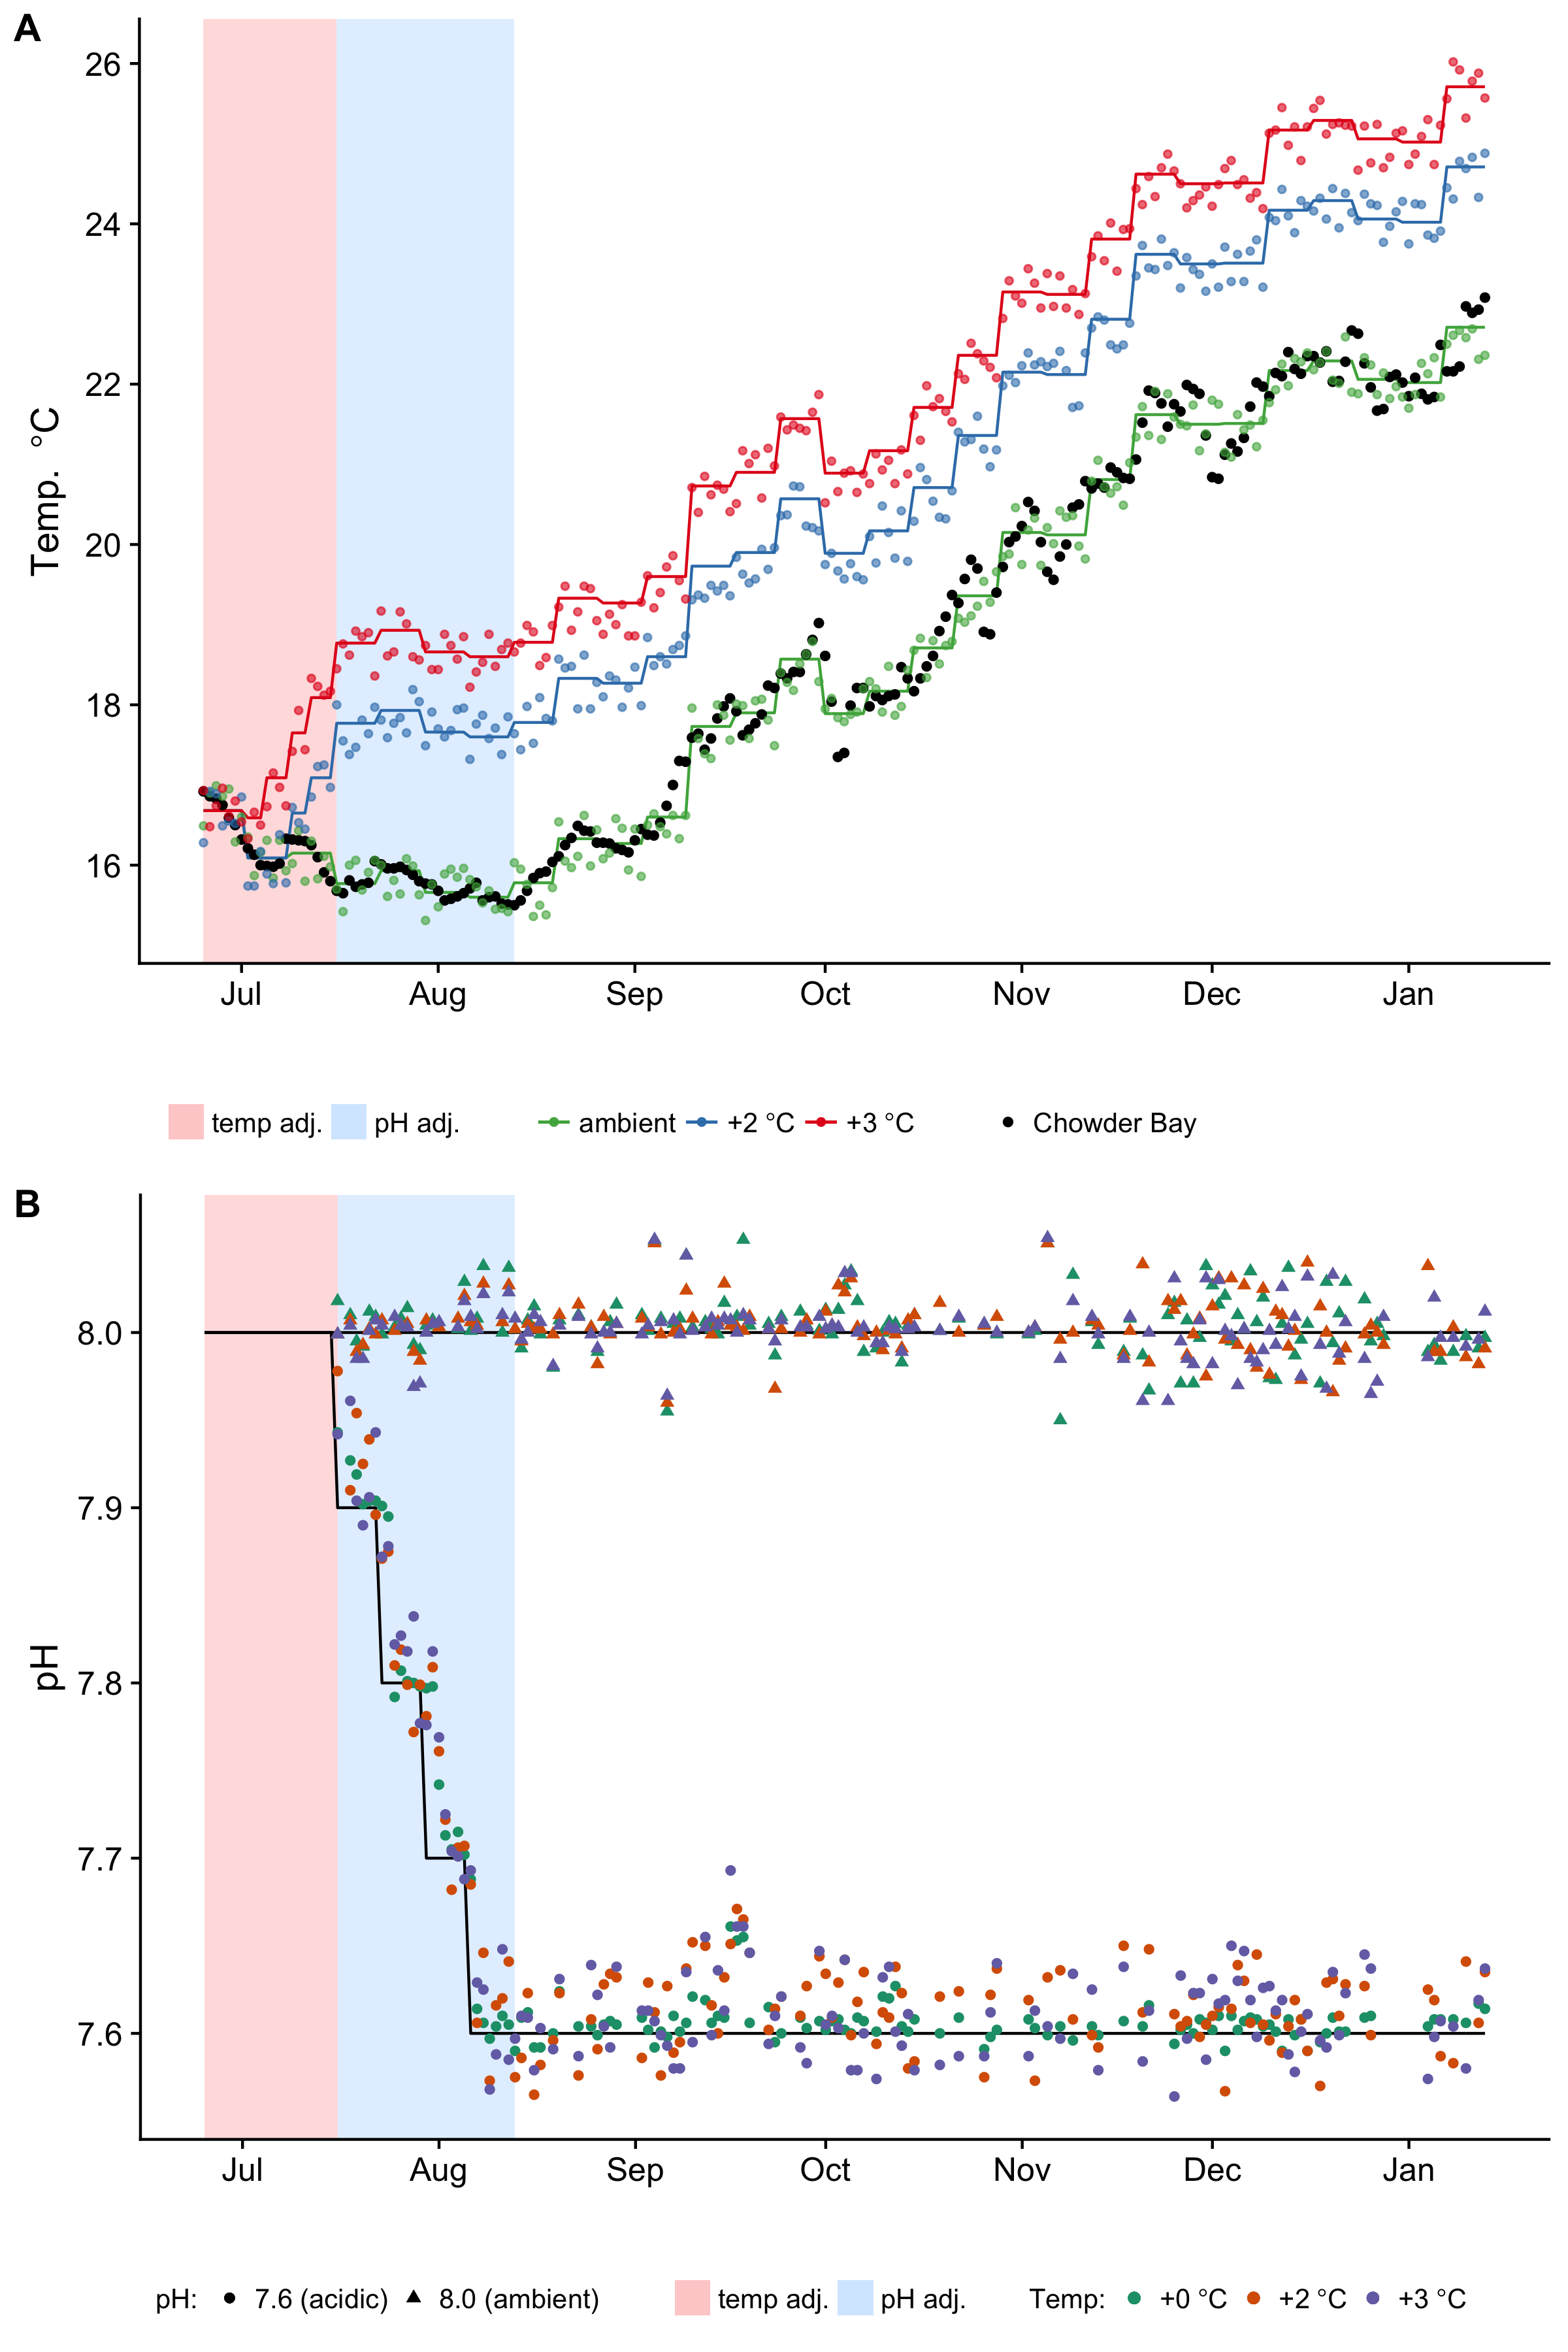
\includegraphics[width=1\linewidth]{figs/ch_multistressor/acclim} \caption{Temperature and pH in treatment tanks, measured daily. Only one replicate tank for every treatment was selected at random for daily measurements. Shaded regions are the pre-acclimation adjustment periods for temperature (pink) and pH (blue), respectively. (A) Coloured lines represent the planned temperature profiles (+0, +2, +3), which change every week, while coloured dots represent the actual temperatures measured. The black dots are the reference temperatures collected from *in situ* loggers deployed in Chowder Bay from 2009 to 2014, averaged by day. (B) Black lines represent the reference constant pH levels, with the initial adjustments (8.0, 7.6). Shapes represent the pH treatment group (triangle: 8.0; circle: 7.6), colours represent the temperature treatment group (+0, +2, +3).}\label{fig:acclim}
\end{figure}

\begin{Shaded}
\begin{Highlighting}[]
\NormalTok{knitr}\OperatorTok{::}\KeywordTok{include_graphics}\NormalTok{(}\StringTok{"figs/ch_multistressor/harbour.png"}\NormalTok{)}
\end{Highlighting}
\end{Shaded}

\begin{figure}
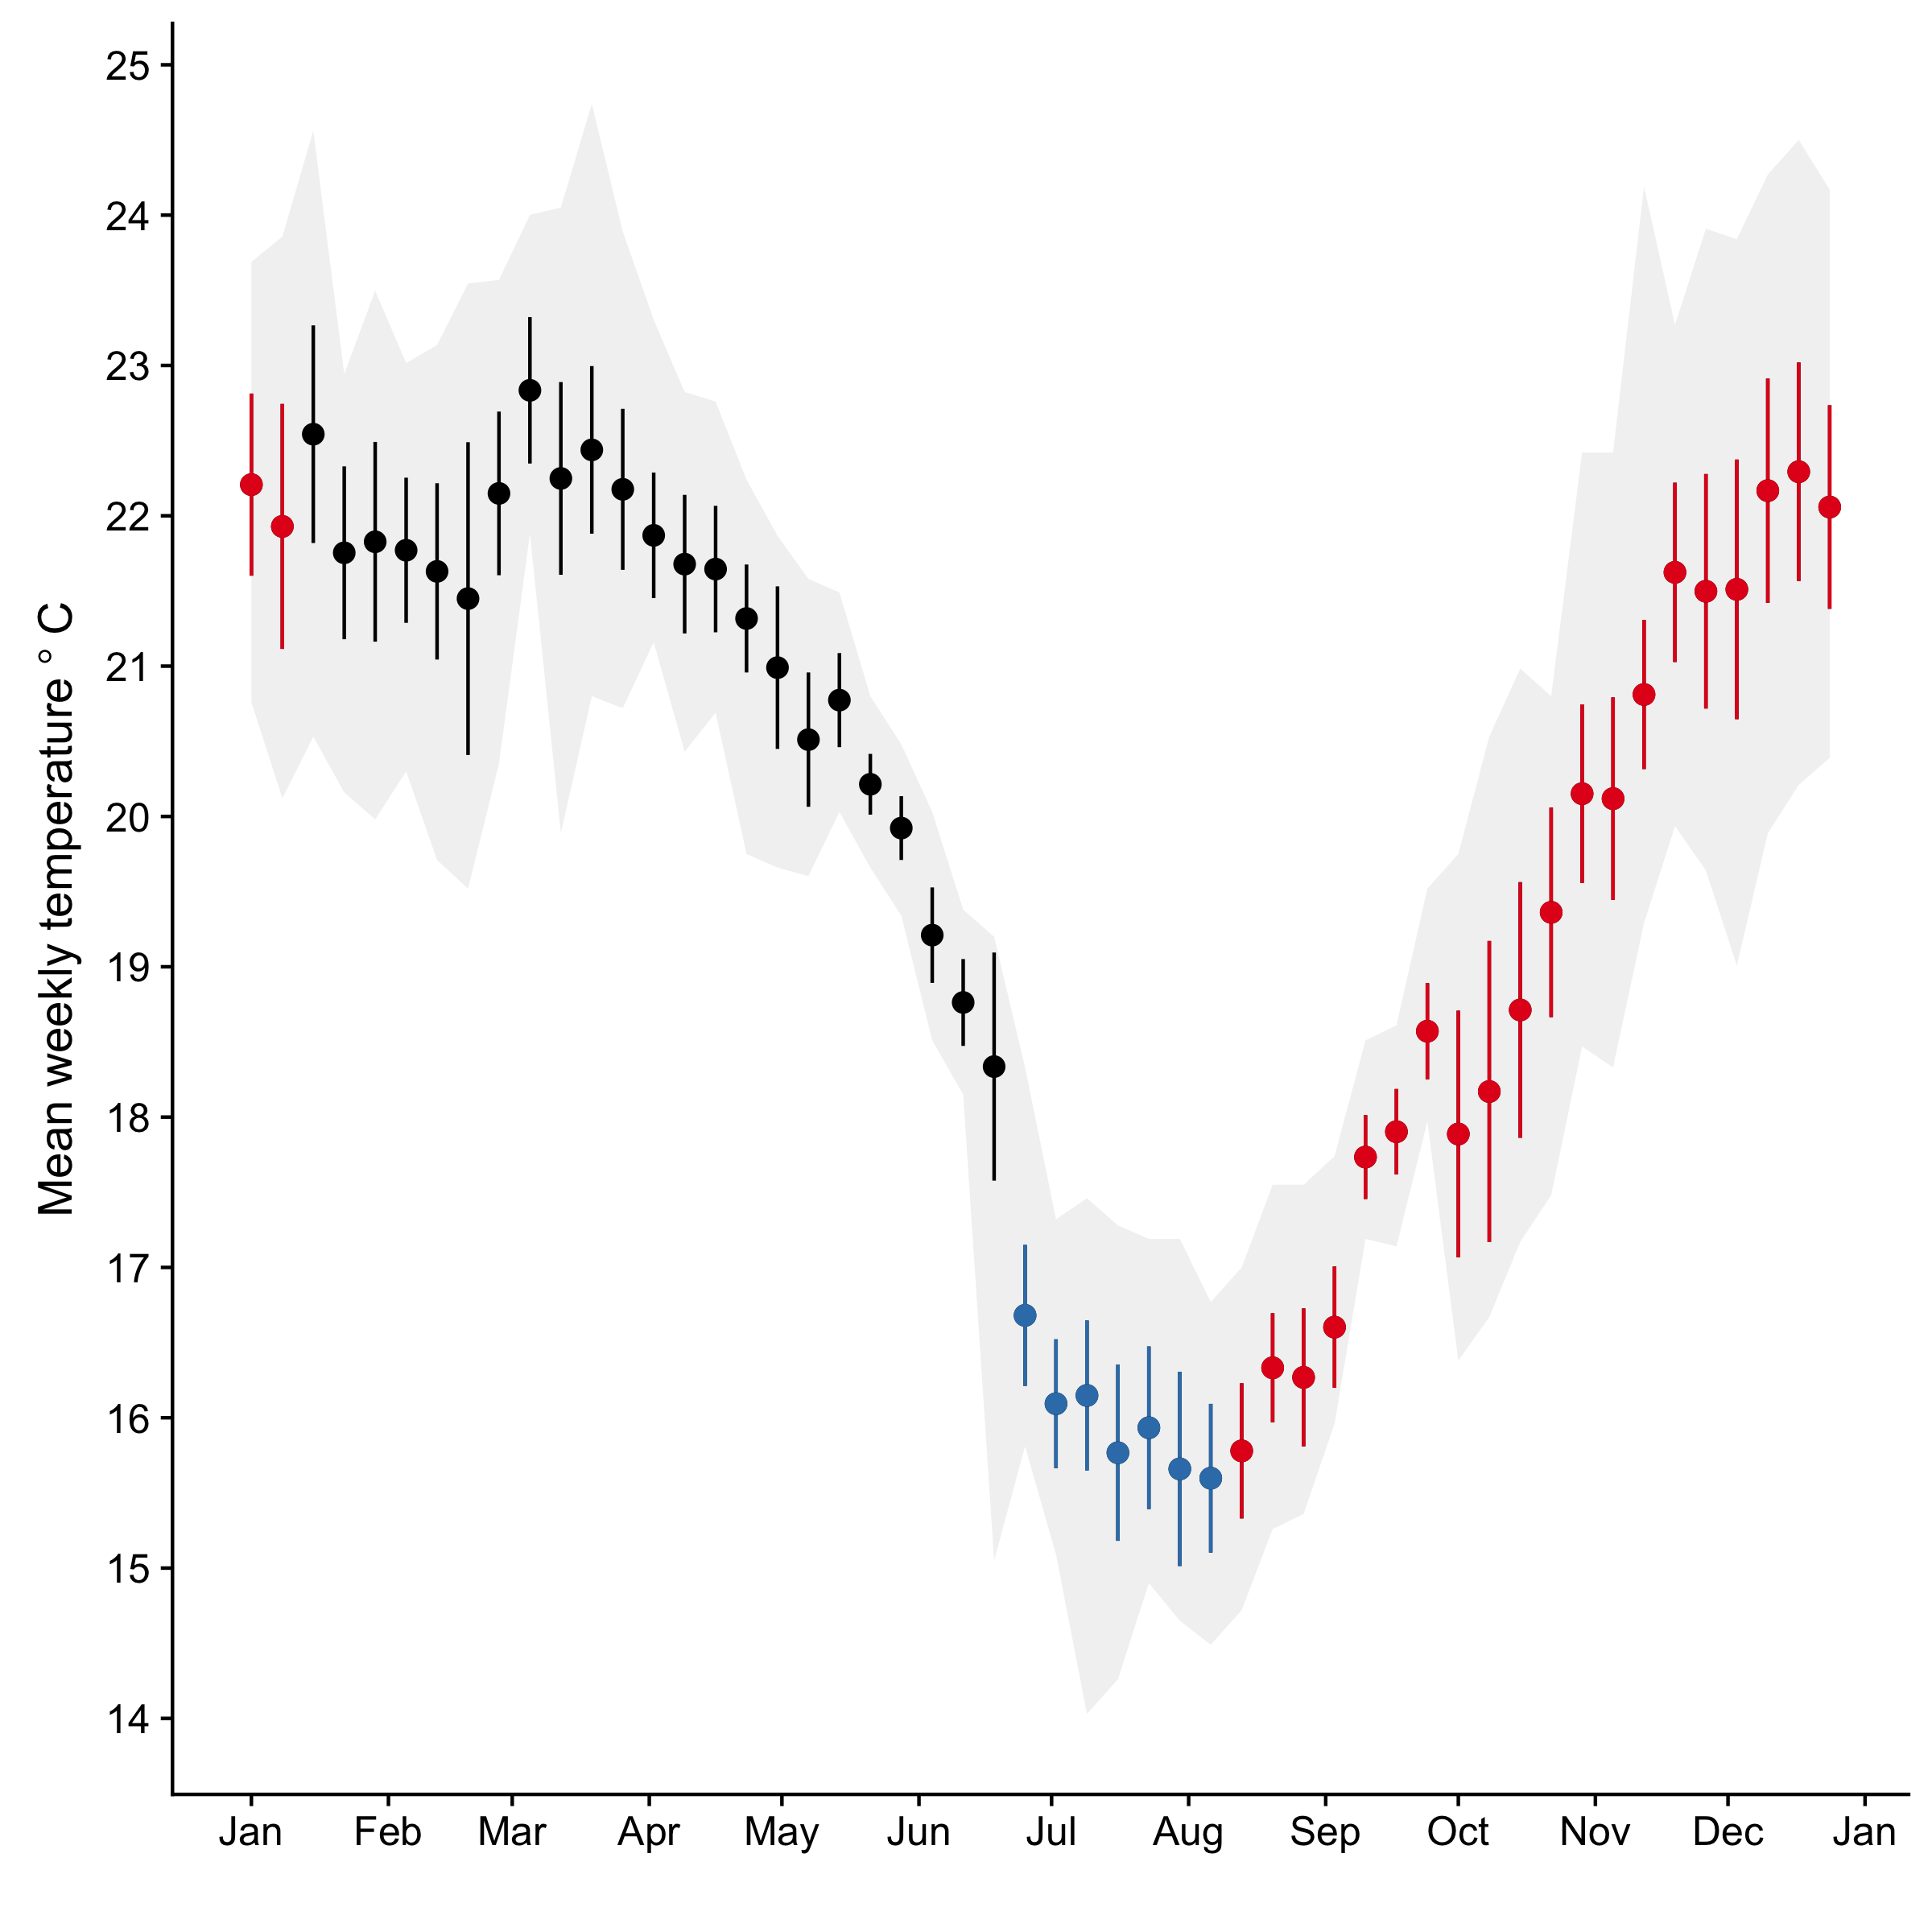
\includegraphics[width=1\linewidth]{figs/ch_multistressor/harbour} \caption{Mean weekly-averaged temperature ($\pm$ s.d.) for Chowder Bay, NSW, Australia, from 2009 to 2014. Data were obtained from loggers deployed *in situ* at 3 m depth at the level of the sea urchin habitat. Colours represent the adjustment (blue) and acclimation (red) periods of the experimental treatments, respectively. The shaded region is the max/min of the temperatures recorded. These data were used to design the temperature profile of the elevated temperature treatments.}\label{fig:harbour}
\end{figure}

\subsection{Monitoring}\label{monitoring}

Temperature was recorded daily in all tanks. Sea water pH was measured
spectrophotometrically with a custom-built sampling system connected to
an Ocean Optics USB4000+ fibre optic spectrometer, using m-Cresol dye
indicator (Acros Argonics, catalog number 110585000, Lot A0321770) and
calculated according to Liu et al. (2011). The measurements were
calibrated to certified reference material (CRM) for \(CO_2\) in
seawater (Batch 139) following SOP 6b in Dickson et al. (2007). The pH
of the tanks were measured every 2 to 3 days. In addition, the sampling
system automatically measured pH in one ambient and one low pH treatment
every two hours to characterise pH during the acclimation period
(Supplementary Material \#\#).

To estimate total alkalinity (\(A_T\)) of the sea water, water samples
(330 mL) were taken randomly from experimental tanks every 2 to 3 weeks
(total \(n = 64\) samples). \(A_T\) was determined by potentiometric
titration (907 Titrando, Metrohm), calibrated using sea water CRMs
(Batch 139; Dickson et al., 2007). The carbonate chemistry parameters
\(pCO_2\), calcite and aragonite staturation states (\(\Omega Ca\) and
\(\Omega Ar\)) were calculated by running the data in the
\enquote{seacarb} package in R (Lavigne et al., 2011) using the
dissociation constants of Mehrbach et al. (1973) refitted by Dickson \&
Millero (1987).

\subsection{Maintenance}\label{maintenance}

Specimens were fed on a diet mixture of fresh \emph{Ecklonia radiata}
and \emph{Sargassum} spp. suspended in kelp-based agar (MSC CO,
Kyeongnam, Korea). To prepare the food, \emph{E. radiata}, and
\emph{Sargassum} spp. were washed in fresh water, dried at
\(50^{\circ}C\) over 48 hours, and then ground into fine powder for
storage. The food was mixed with agar powder to a ratio of 1:4 by
weight, and then mixed with FSW (20 \(\mu m\)) to a ratio of 1:10 by
weight at \(\sim 80 ^{\circ}C\). The agar was left to cool and solidify
for 45 minutes, before it was cut into 1 to 2 \(cm^2\) cubes and fed to
the specimens. We fed the specimens twice a week by placing 3 to 4 cubes
on top of each individual urchin. This feeding technique ensured that
each animal received the same amount of food in excess during the entire
experimental period.

All treatment tanks were siphoned every two days and wiped weekly to
remove faecal matter and minimise algal growth. \(CO_2\) diffusers were
scrubbed and replaced every 3 to 5 days. Header tanks were cleaned of
algal growth once a month.

\subsection{Survival}\label{survival}

Survival was recorded by measuring the survival time of individual
specimens for 155 days (Aug--Dec 2014). Specimens were observed daily
for mortality, and dead urchins were removed immediately.

\subsection{Metabolic rate}\label{metabolic-rate}

Routine weight-specific metabolic rate, \(MO_2\) was estimated by
intermittent-flow respirometry at two time-points (at 4 and 12 weeks of
acclimation), from a random subsample of specimens
(\(n = 10\ treatment^{-1}\)). The specimens were not fed for 5 days
prior to measurements and transferred individually into \(1\ L\)
respirometry chambers. Each respirometry chamber was kept in an
individual water bath and contained an oxygen sensor spot (SP-PSt3-NAU,
PreSens GmbH, Germany) for the detection of dissolved oxygen
concentration using an external multi-channel sensor (OXY-10-mini,
PreSens Gmbh, Germany). A magnetic stirrer ensured even mixing of water.
The specimens were allowed to adjust to the chambers under flow-through
conditions for 30 minutes prior to respirometry measures.

To measure oxygen uptake, chambers were sealed and dissolved oxygen (DO,
\(mgO_2\ L^{-1}\)) was measured every 10 seconds until a 10\% decrease
in DO was recorded. The chamber was then flushed, and the measurement
repeated. Background respiration was determined by recording FSW-only
blanks (\(n\) = 8) to correct the recordings for background respiration
and instrument drift. At the end of each measurement, sea water weight
was calculated by deducting chamber, stir bar and urchin wet weights
from the total weight of the chamber, and then converted to volume using
sea water density estimated from current temperature, salinity and
barometric air pressure (Fofonoff \& Millard 1983).

Weight-specific \(MO_2\) (\(mgO_2\ L^{-1}\ h^{-1}\)) was calculated
using the equation (Lighton 2008):

\begin{equation}
  MO_2 = \frac{\Delta O_2V}{W}
  \label{eq:mo2}
\end{equation}

\noindent where \(\Delta O_2\) is the linear regression of \(O_2\)
concentration over time (\(mg\ L^{-1}\ h^{-1}\)), \(V\) is the volume of
the sea water available (\(L\)) and \(W\) is the wet weight of the
urchin (\(g\)).

\subsection{Feeding rate and assimilation
efficiency}\label{feeding-rate-and-assimilation-efficiency}

Feeding trials were conducted after 13 weeks of acclimation. Specimens
were transfered into individual tanks (\(4\ L\)) supplied with
flowthrough FSW (\(6\ L\ h^{-1}\)) at the same treatment conditions.
They were starved for 6 days in their new environments before feeding
trials commenced, using the same agar-based food mixture used in routine
feeding. Initial wet weight of the diet was determined and food was
added to each tank in excess. Food-only autogenic controls were used to
determine background changes in agar composition (\(n = 24\)).

After 48 hours, unconsumed food was carefully collected and oven dried
at \(80^{\circ}C\) for 48 h, and then re-weighed. Faecal pellets were
also siphoned at the same time for calculations of assimilation
efficiency (see below). The specimens were removed from the tanks,
blotted briefly with paper towel, and weighed. To convert the initial
wet weight (\(W_{wet}\)) of the food to their dry-weight equivalents,
the wet:dry ratio of the food was determined in a regression analysis of
wet to dry weights (\(n = 60\), \(r^2 = 0.82\), \(p < 0.01\)), and
determined as:

\begin{equation}
  W_{dry} = (0.1529 \times W_{wet}) - 0.036
  \label{eq:wdry}
\end{equation}

Feeding rate, \(C\) (\(mg\ day^{-1}\ kg^{-1}\)), was calculated by
subtracting the final dry weight (\(W_{T1}\)) from the initial dry
weight (\(W_{T0}\)), with adjustments for background changes and
specimen weight (\(W_{sp}\)) and adjusted by time (\(T\)):

\begin{equation}
  C = \frac{W_{T0} - W_{T1}}{W_{sp} \cdot T}
  \label{eq:c}
\end{equation}

Faecal samples were dried at \(60^{\circ}C\) for 48 hours and weighed.
These samples were then ashed in a muffle furnace at \(500^{\circ}C\)
for 2--3 hours and re-weighed to determine their ash-free dry weight
(AFDW). Assimilaiton efficiency (\%) was calculated using the Conover
method (Conover, 1966):

\begin{equation}
  A = \left[ \frac{F - E}{(1 - E) \cdot F} \right] \times 100\%
  \label{eq:a}
\end{equation}

where \(F\) and \(E\) denote the AFDW:dry weight fraction measured in
the diet and the faeces, respectively. All weights were determined using
the same analytical balance accurate to 0.0001 g.

\subsection{Ammonia excretion}\label{ammonia-excretion}

To determine ammonia excretion rate 10 randomly selected specimens from
each treatment that had not been used for respirometry were placed in
the respirometry chambers (total \(n = 60\)). Initial water samples were
carefully collected (\(50 mL\), \(0.22 \mu m\)). The chambers were
sealed and left in the water baths for 3 hours before final water
samples were collected. Background ammonia levels were determined by
repeating the experiment without specimens (\(n = 3\ treatment^{-1}\)).
The water samples were immediately frozen and stored in the dark until
they were analysed spectrophotometrically (within 10 days) for total
ammonia, following the methods of Parsons et al. (1984).
Spectrophotometric readings were obtained at 640 nm on a microplate
reader (CLARIOstar Microplate Reader, BMG LABTECH, Offenburg, Germany)
and calibrated using daily blanks and a standard ammonium solution
(Parsons et al., 1984). Ammonia excretion rate, \(U\)
(\(\mu g\ kg^{-1}\ h^{-1}\)) was calculated according to the equation:

\begin{equation}
  U = \frac{N_c}{W \cdot T}
  \label{eq:u}
\end{equation}

where \(N_c\) is the concentration of ammonia
(\(\mu g\ at\mbox{-}N\ L^{-1}\)), \(W\) is the weight of the specimen in
\(kg\) and \(T\) is the time elapsed in hours. Ammonia concentration,
\(N_c\) is determined following Parsons et al. (1984) and is summarised
in the equation:

\begin{equation} 
  N_c = \frac{3 \cdot V}{\Delta E}
  \label{eq:nc}
\end{equation}

where \(\Delta E\) is the difference between the standard and corrected
spectrophotometric extinction values of the blue indophenol colour
formed with ammonia and \(V\) is the volume of the chamber (\(L\)).

\subsection{Scope for growth (SfG)
parameters}\label{scope-for-growth-sfg-parameters}

To explore the influence of temperature and pH stressors on the growth
potential of \emph{H. erythrogramma}, we constructed a SfG model using
data from respirometry, feeding trials and ammonia analyses.

Oxygen consumption was converted to energy equivalent values to
calculate the energy lost in respiration per day, \(R_E\), using a
conversion factor of \(14.14 J\ mg^{-1}\ O_2\) (Elliot and Davidson,
1975). A conversion factor of \(0.025 J\ g^{-1}\) ammonia (Crisp, 1984,
Elliott and Davison, 1975) was used to estimate the energy equivalent of
the energy lost due to ammonia excretion per day, \(U_E\).

The energy available from food, \(C_E\), was calculated using
bomb-calorimetry using an automatic adiabatic bomb calorimeter
(Gallenkamp, London). The calorimeter was calibrated for the heat of
combustion of \(1 g\) of benzoic acid (26.493 \(kJ\ g^{−1}\)) at least
three times to determine the approximate effective heat capacity of both
the bomb chamber and the mass of the water within the calorimeter
chamber, \(C_S\) (10.27 \(\pm\) 0.07 \(kJ\ ^{\circ}C\)).

The diet was dried in an oven at \(60^{\circ}C\) to remove moisture.
Approximately 1 \(g\) of the diet was used each time to determine gross
energy via combustion, and the experiment was repeated six times to
obtain an average value (12.67 \(\pm\) 0.25 s.d. \(kJ\ g^{-1}\)) using
the equation:

\begin{equation}
  C_E = \frac{\Delta T \times C_S}{W_S}
  \label{eq:ce}
\end{equation}

where \(\Delta T\) \((^{\circ}C)\) is the change in temperature --
detected using a Beckmann thermometer -- between the initial and
post-combustion of the sample, \(C_S\) is the effective heat capacity of
the system (bomb chamber and water), and \(W_S\) is the weight of the
diet sample (\(g\)).

To calculate scope for growth (\(SfG\)) we used the equation adapted
from Winberg (1960):

\begin{equation}
  SfG = C_E \cdot A - (R_E + U_E)
  \label{eq:sfg}
\end{equation}

where \(C_E\) is the energy obtained from diets, \(A\) is the
assimilation efficiency, \(R_E\) is the energy lost in respiration and
\(U_E\) is the energy lost due to ammonia excretion. All energy-related
units are in \(kJ\ g^{-1}\ day^{-1}\), while assimilation efficiency is
a proportion.

We did not follow individual urchins, so the SfG data could not be
analysed using the statistical approach (e.g.). Rather, we constructed
the SfG model using treatment-averaged parameters as an indicative
assessment of the impacts of our acclimation treatments on \emph{H.
erythrogramma}.

\subsection{Statistical analyses}\label{statistical-analyses}

Analyses were performed in R (v 3.4.3). The survival time for each
specimen was determined by the number of days from time zero when the
acclimation period started to the end of the experiment. Survival data
were analysed using Cox proportional hazards models (Cox, 1972), with
right censoring, to determine whether temperature and pH affect survival
time. Two model fits were run:

\begin{enumerate}
\def\labelenumi{\arabic{enumi}.}
\tightlist
\item
  Model 1:
  \texttt{(survival\ time)\ \textasciitilde{}\ temperature\ +\ pH\ +\ (temperature\ *\ pH)}
  -- where the interaction between temperature and pH was included; and
\item
  Model 2:
  \texttt{(survival\ time)\ \textasciitilde{}\ temperature\ +\ pH} --
  main effects only.
\end{enumerate}

The fitted Cox regression met the assumption of proportional hazards
(Schoenfeld residual tests, Grambsch and Therneau 1994; \(p = 0.673\)).
As no interactions were found between temperature and pH (Cox,
\(p = 0.54\)), Model 1 was selected to test for main effects.\\
\emph{Post-hoc} tests for the differences between treatments were
determined using pairwise tests of significance corrected using the
Benjamini-Hochberg (BH) false discovery rate method (Benjamini and
Hochberg, 1995).

Metabolic rate data were analysed by constructing a linear model of
metabolic rate as a function of temperature (\(+0^{\circ}C\),
\(+2^{\circ}C\), \(+3^{\circ}C\)), pH (8.0, 7.6) and time (4 weeks, 12
weeks) as fixed factors. Feeding rate data were analysed by constructing
a linear model of feeding rate as a function of temperature and pH as
fixed factors. To test for effects, ANOVA was performed on the models,
using type III sums of squares when interactions were present, or type
II sums of squares when they were not (Langsrud 2003). For metabolic
rate data, the ANOVA revealed no significant interactions between
acclimation time, temperature and pH (\(F_{2,104}= 2.37\),
\(p = 0.098\)). Thus, the three-way interaction term was removed from
the model and the data re-analysed to only test for two-way interactions
and single effects. All analyses were tested for normality and
homogeneity of variances. Where treatment conditions were indicated to
be significantly different, estimated marginal means (EMM, aka
Least-Squares Means) were used to develop linear estimates for the
post-hoc Tukey Highest Significant Difference (HSD) test to identify the
significance between metal-tissue combinations. Significance was
determined at p \textless{} 0.05 or lower for all statistical tests.

As different individual urchins were used to provide some of the
parameters used to construct the model, SfG was calculated based using
treatment-averaged parameters. Thus, we were unable to perform
statistical tests of significant differences in SfG between treatment
groups.

\section{Results}\label{results}

\subsection{Survival}\label{survival-1}

There was a significant effect of treatment condition on survival
response (\emph{logrank test}, \(\chi_2\) = 61.23, \(d.f. =\) 3, \(p\)
\textless{} 0.001) with no interaction between temperature and pH (Cox
regression, \(z =\) 0.61, \(d.f. =\) 3, \(p =\) 0.54). As single
stressors, decreased pH did not significantly affect survival
(\(p\ = 0.296\), HR: 0.46, 95\% CI: 0.10 -- 1.99), neither did a
\(+2 ^{\circ}C\) increase in temperature (\(p = 0.146\), HR: 2.68, 95\%
CI: 0.71 -- 10.09). For these treatments, survival was \(>80\%\) after
155 days. At \(+3 ^{\circ}C\), survival decreased significantly
(\(p < 0.001\), HR: 17.2, 95\% CI: 5.27 -- 56.25) regardless of pH level
(pH 8.0: 40\%; pH 7.6: 33\%). These \(+3^{\circ}C\) treatments were the
only ones that crossed the median surival threshold after 155 days
(Figure \ref{fig:surv}). \emph{Post-hoc} results (pairwise tests,
BH-corrected) showed that urchins acclimated to \(+3 ^{\circ}C\) had
significantly lower survival compared to all other treatments (\(p <\)
0.01 for all pairwise combinations), with no significant differences in
other pairwise comparisons.

\begin{Shaded}
\begin{Highlighting}[]
\NormalTok{knitr}\OperatorTok{::}\KeywordTok{include_graphics}\NormalTok{(}\StringTok{"figs/ch_multistressor/surv_plot.png"}\NormalTok{)}
\end{Highlighting}
\end{Shaded}

\begin{figure}
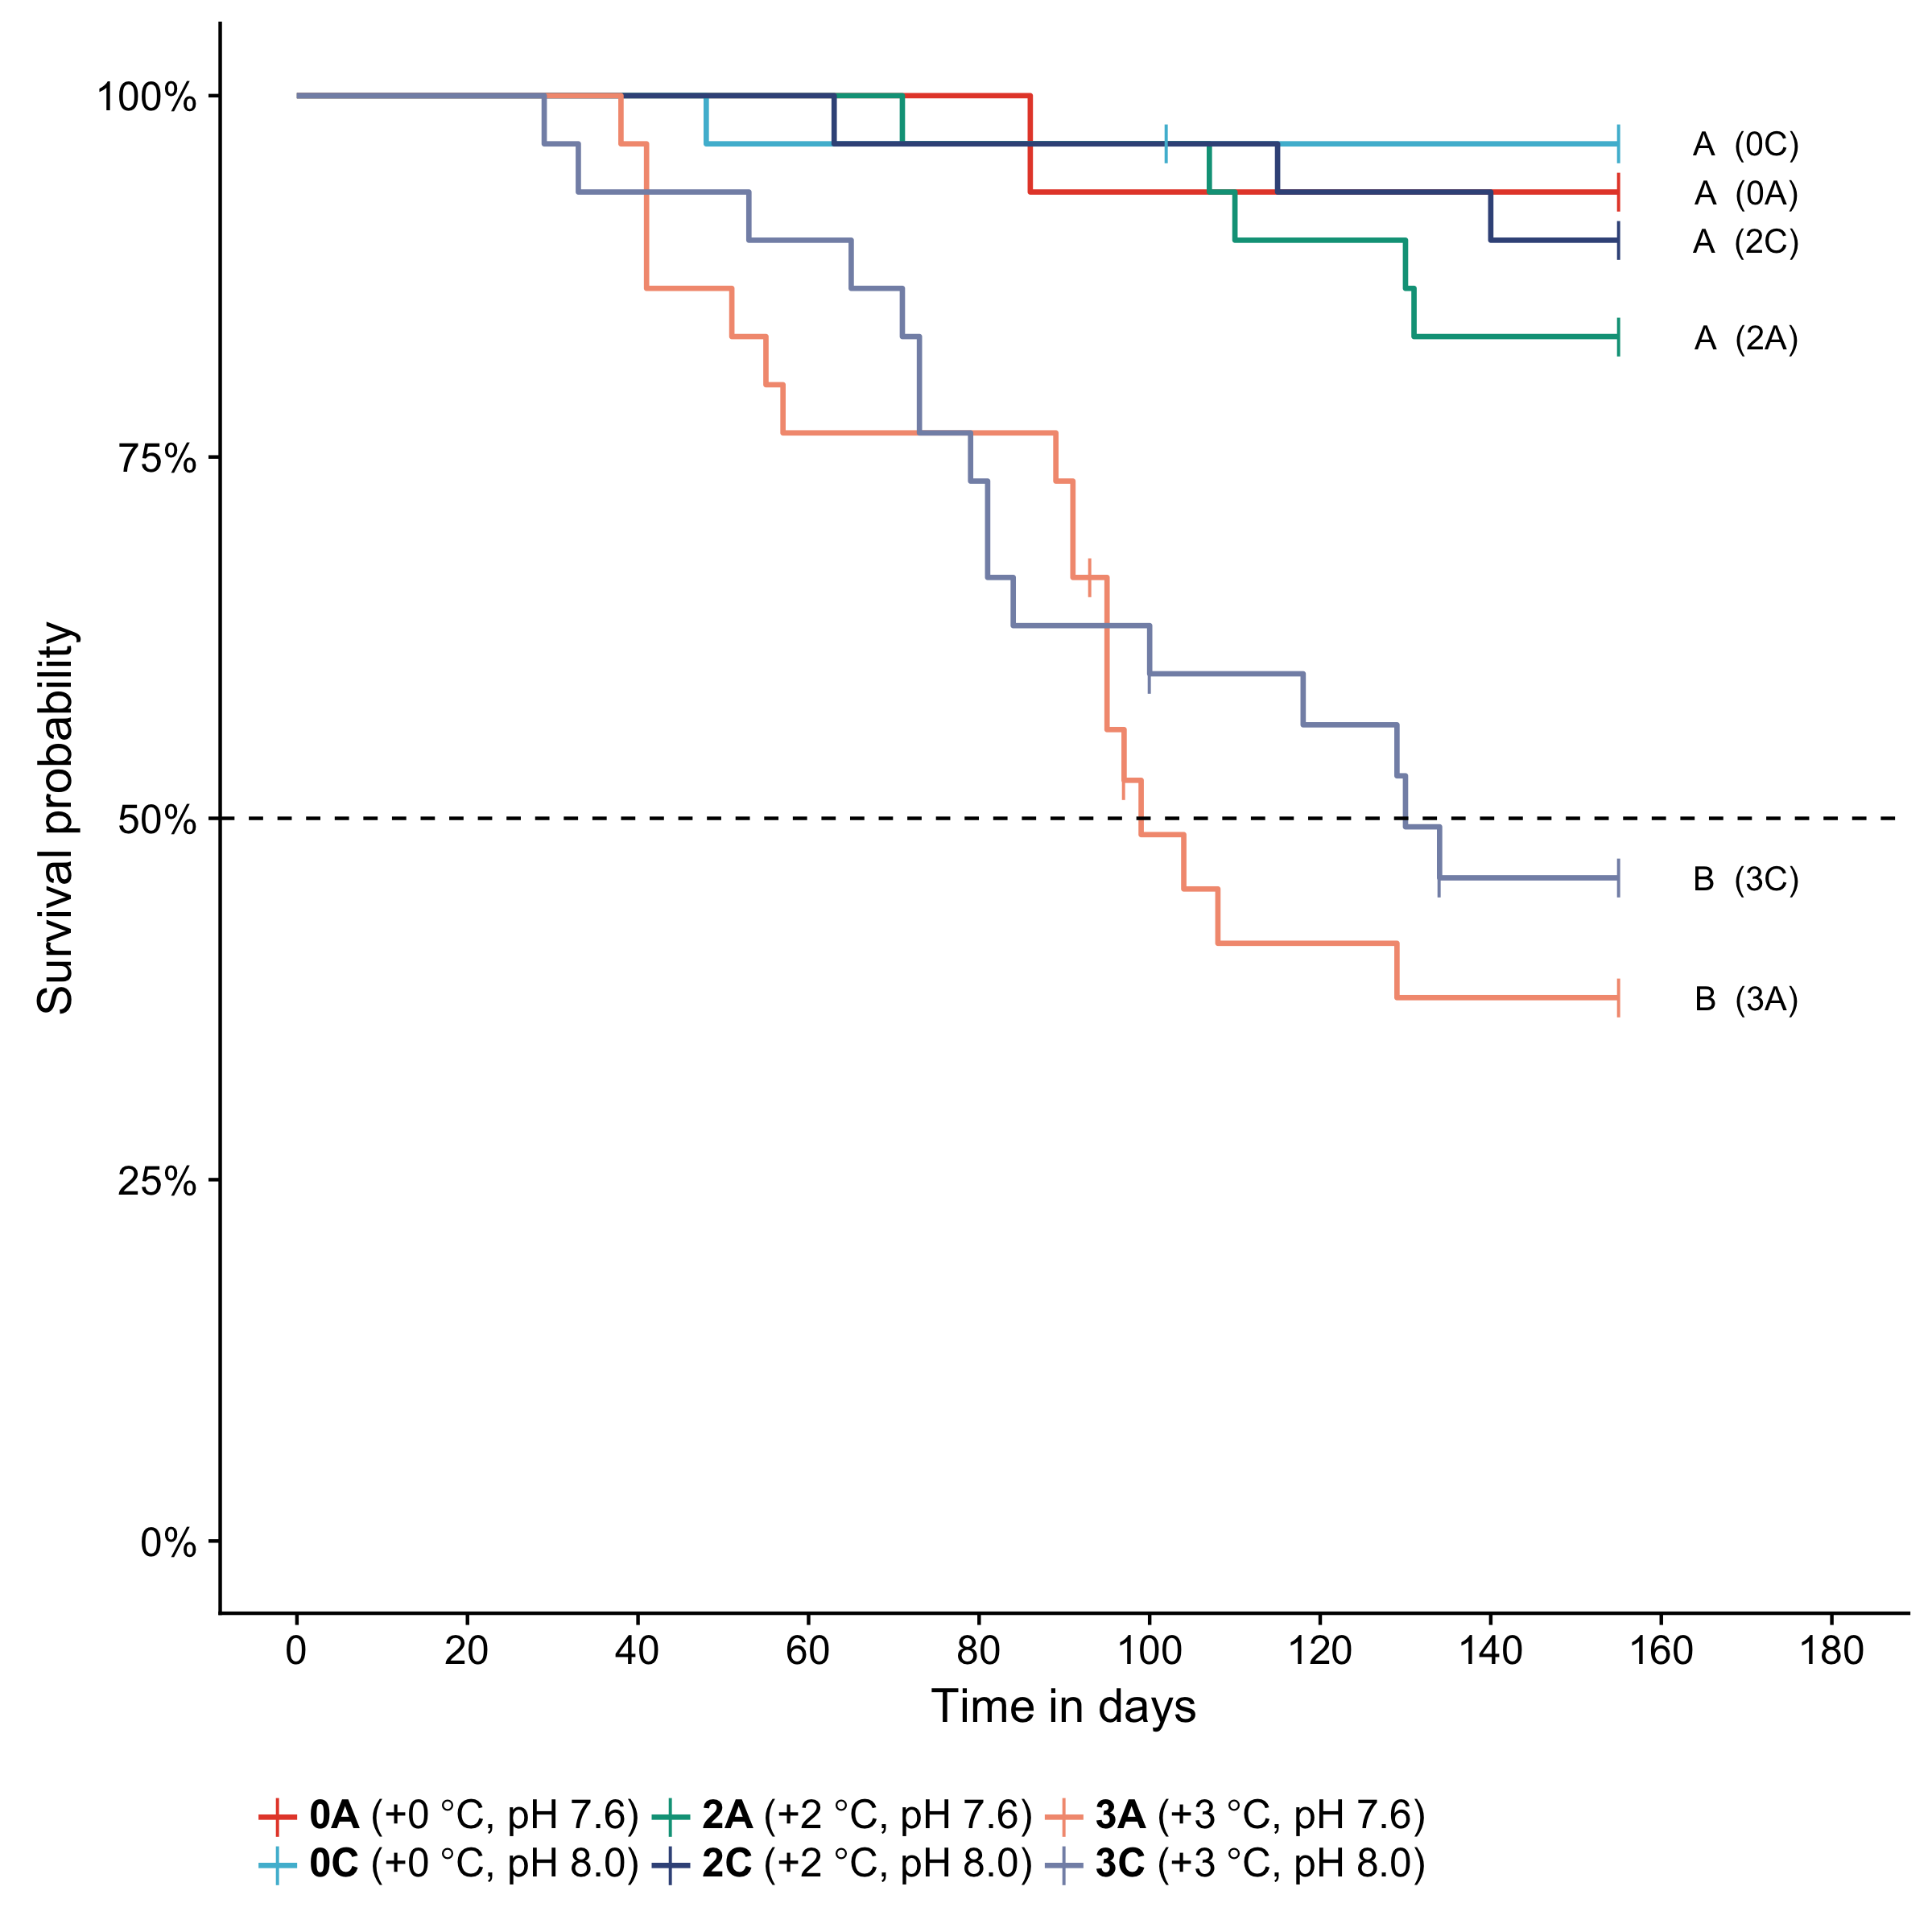
\includegraphics[width=1\linewidth]{figs/ch_multistressor/surv_plot} \caption{Survival in *H. erythrogramma* acclimated to combinations of increased temperature (ambient +0, +2, $+3 ^\circ C$) and decreased pH (ambient 8.0, decreased 7.6). Letters indicate treatments that differed (pairwise tests, with Benjamini-Hochberg (BH) false discovery rate corrections, p < 0.05).}\label{fig:surv}
\end{figure}

\subsection{Metabolic rate}\label{metabolic-rate-1}

The 2-way ANOVA showed that there were significant two-way interactions
for acclimation time\(\times\)pH (\(F_{1,106}= 10.7\), \(p = .001\)),
temperature\(\times\)pH (\(F_{5,106}= 3.36\), \(p = 0.039\)), and
acclimation time\(\times\)temperature (\(F_{2,106}= 14.1\),
\(p < 0.001\)). As single stressors, increased temperature
(\(F_{2,106}= 8.69\), \(p < .001\)) and decreased pH
(\(F_{1,106}= 22.8\), \(p < .001\)) significantly influenced metabolic
rate.

Results of \emph{post-hoc} analyses using Tukey's HSD showed that
although acclimation time alone did not significantly affect metabolic
rate (\(F_{1,106}= 1.42\), \(p = 0.24\)), it clearly interacted with
temperature or pH. At 4 weeks of acclimation, metabolic rate increased
significantly as a result of elevated temperature
(\(p = < 0.0001\)--\(0.08\)) or decreased pH (\(p < 0.001\)).

but at 12 weeks of acclimation, there were no significant pairwise
differences between any treatment combinations.

\begin{Shaded}
\begin{Highlighting}[]
\NormalTok{knitr}\OperatorTok{::}\KeywordTok{include_graphics}\NormalTok{(}\StringTok{"figs/ch_multistressor/resp_plot.png"}\NormalTok{)}
\end{Highlighting}
\end{Shaded}

\begin{figure}
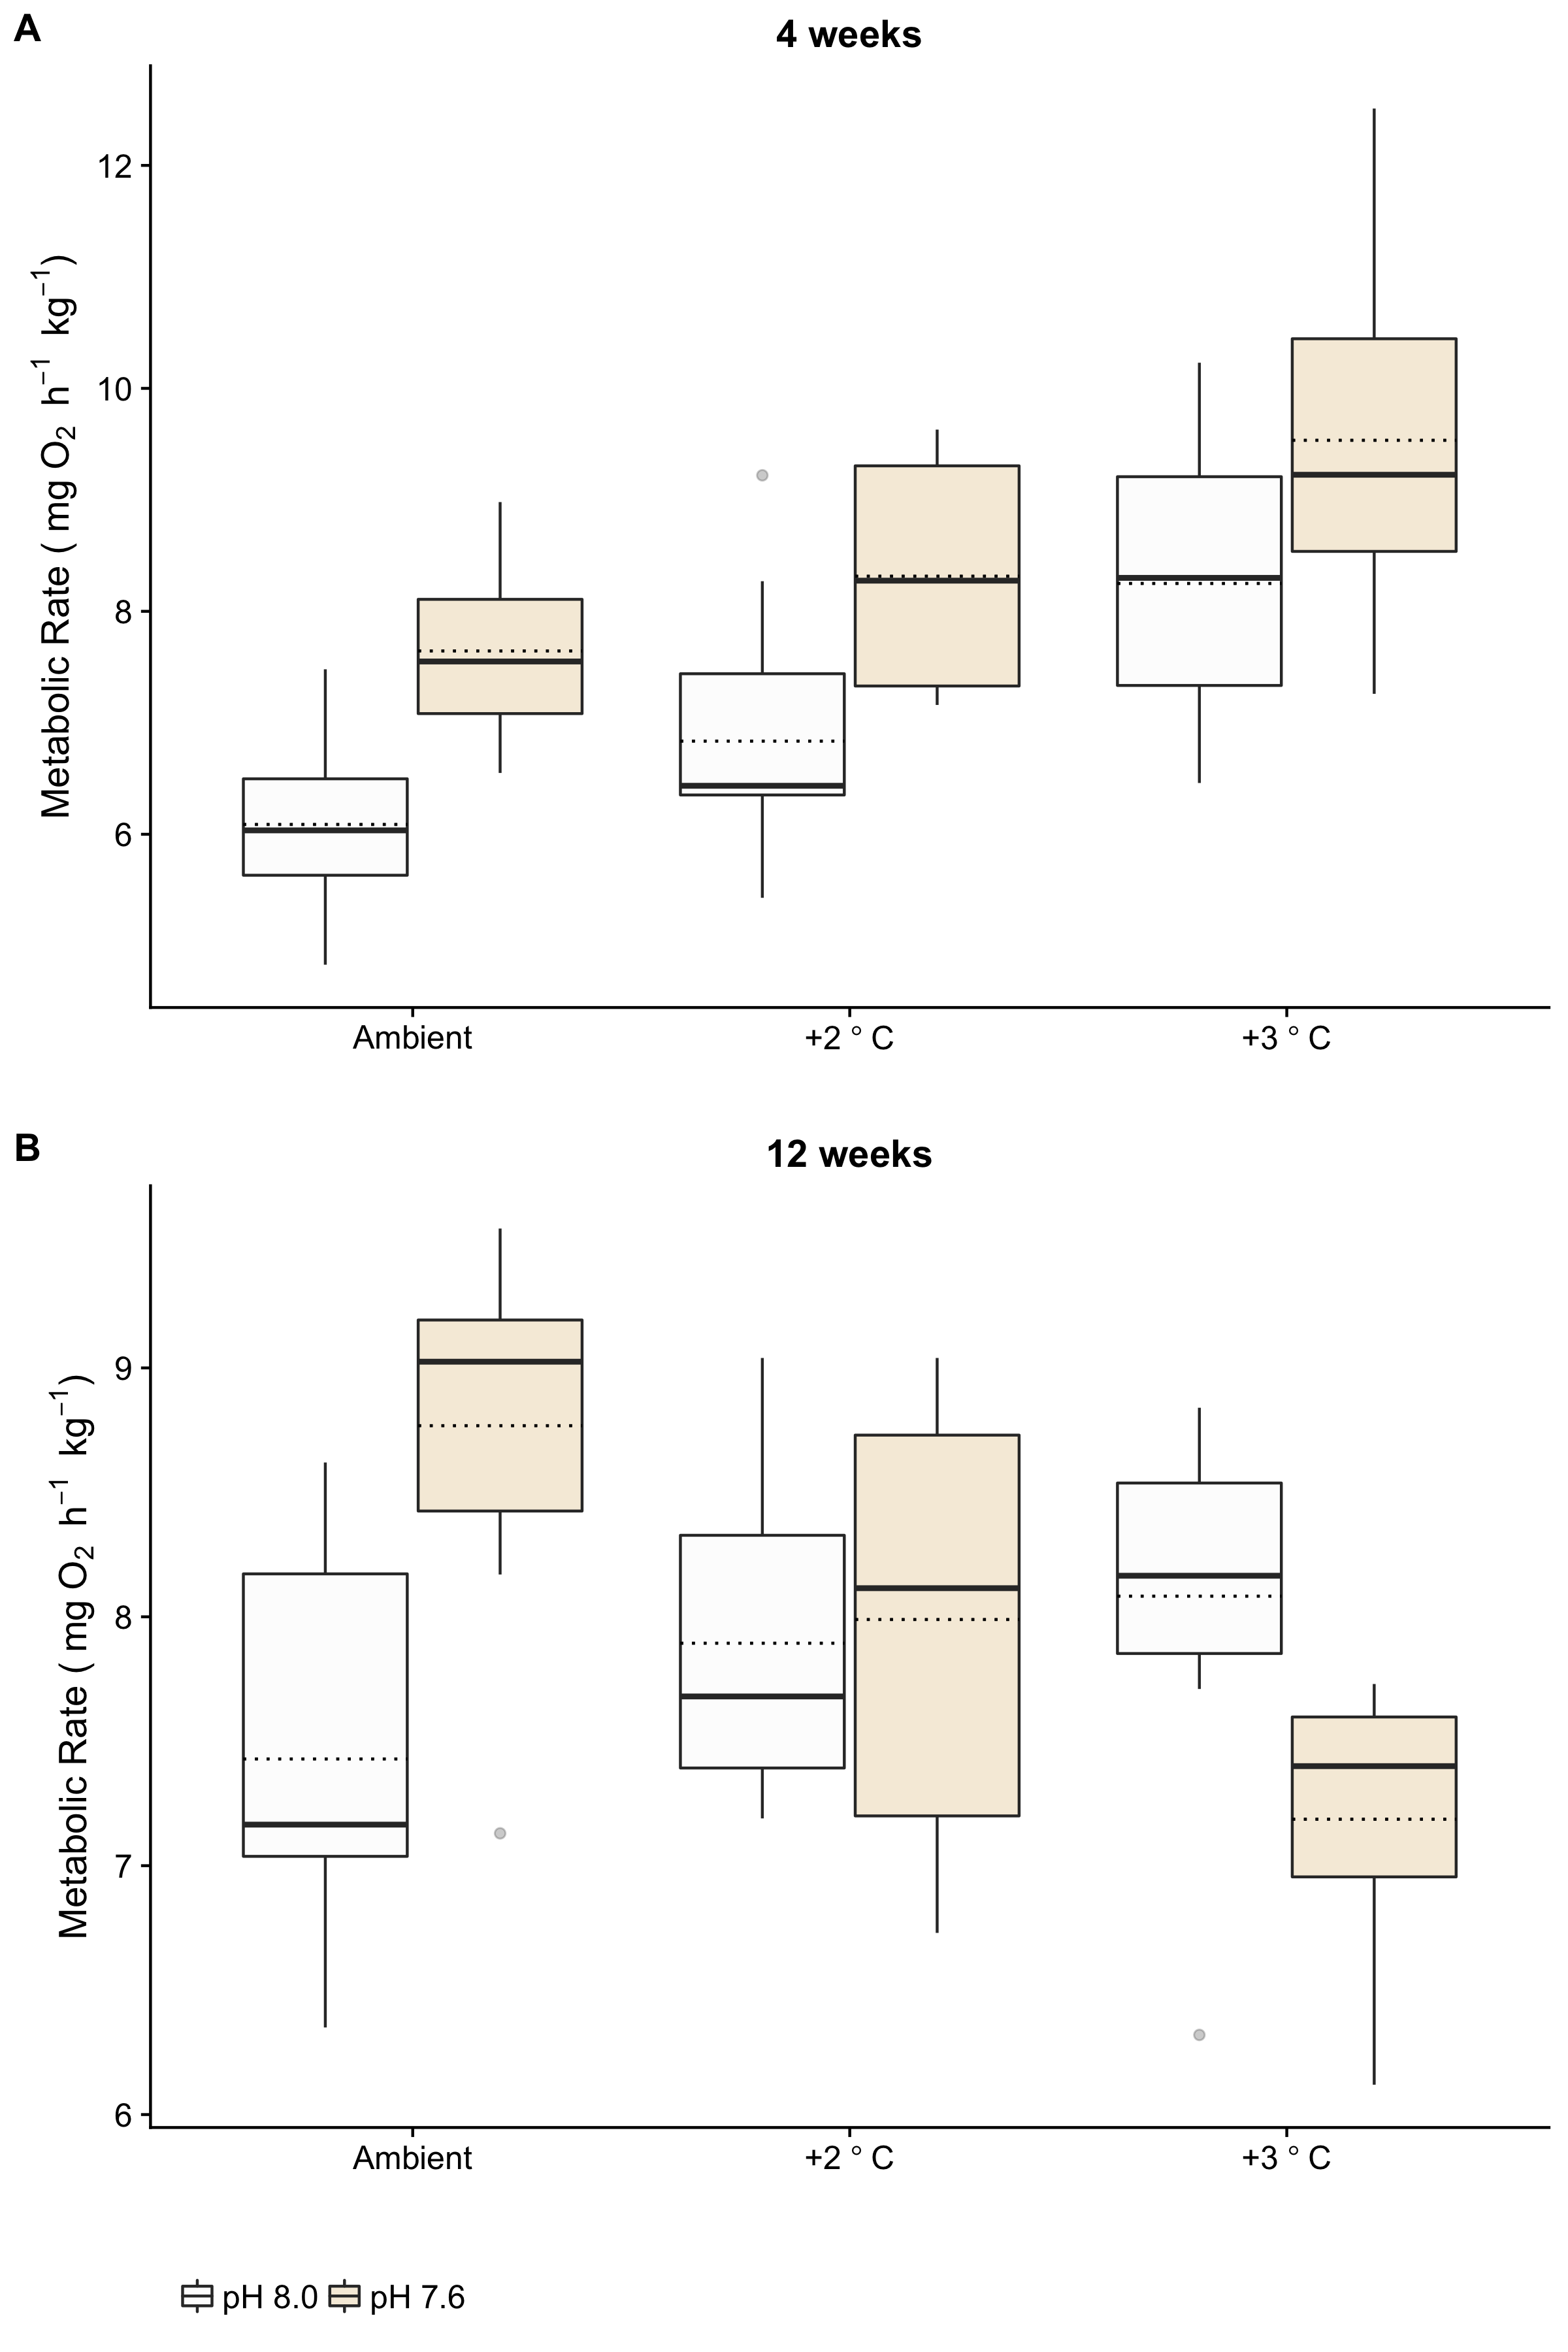
\includegraphics[width=1\linewidth]{figs/ch_multistressor/resp_plot} \caption{Metabolic rate of *H. erythrogramma* acclimated for 12 weeks in six treatments of three temperatures ($+0, +2, +3 ^\circ C$) and two pH levels (8.0, 7.6). The top and bottom of the boxes represent the interquartile range (IQR) between the 25th and 75th percentile (Q1 and Q3, respectively). The horizontal line represents the median (Q2), the horizontal dotted line represents the mean, and the vertical lines (whiskers) represent the range of the data computed as follows: Q1 − 1.5IQR (bottom whisker); greater than Q3 + 1.5 IQR (top whisker).}\label{fig:resp}
\end{figure}

\subsection{Feeding rate and assimilation
efficiency}\label{feeding-rate-and-assimilation-efficiency-1}

The 2-way ANOVA showed that feeding rate was significantly influenced by
elevated temperature (\(F_{2,90} = 10.88\), \(p < 0.001\)), but not pH
(\(F_{2,90} = 0.02\), \(p = 0.9\)). There were also no statistically
significant interactions between temperature and pH
(\(F_{2,90} = 1.15\), \(p < 0.32\)). Acclimation to increased
temperature of \(+2 ^\circ C\) and \(+3 ^\circ C\) significantly
decreased feeding at pH 7.6 (p = 0.001 and p = 0.008, respectively), but
not at pH 8.0. No other significant differences were detected.

\begin{Shaded}
\begin{Highlighting}[]
\KeywordTok{load}\NormalTok{(}\StringTok{"output/ch_multistressor/feeding.RData"}\NormalTok{)}
\NormalTok{hsd}\OperatorTok{$}\NormalTok{contrasts}
\end{Highlighting}
\end{Shaded}

\begin{verbatim}
## ph = pH 8.0:
##  contrast       estimate         SE df t.ratio p.value
##  amb - high  0.040364781 0.01835533 90   2.199  0.0768
##  amb - med   0.030802658 0.01835533 90   1.678  0.2192
##  high - med -0.009562123 0.01835533 90  -0.521  0.8613
## 
## ph = pH 7.6:
##  contrast       estimate         SE df t.ratio p.value
##  amb - high  0.069437422 0.01835533 90   3.783  0.0008
##  amb - med   0.068344931 0.01835533 90   3.723  0.0010
##  high - med -0.001092490 0.01835533 90  -0.060  0.9980
## 
## P value adjustment: tukey method for comparing a family of 3 estimates
\end{verbatim}

\begin{Shaded}
\begin{Highlighting}[]
\NormalTok{grps}\OperatorTok{$}\NormalTok{contrasts}
\end{Highlighting}
\end{Shaded}

\begin{verbatim}
##     contrast     ph     estimate         SE df     t.ratio      p.value
## 3 high - med pH 8.0 -0.009562123 0.01835533 90 -0.52094515 0.8613221099
## 2  amb - med pH 8.0  0.030802658 0.01835533 90  1.67813110 0.2191683756
## 1 amb - high pH 8.0  0.040364781 0.01835533 90  2.19907625 0.0767762508
## 6 high - med pH 7.6 -0.001092490 0.01835533 90 -0.05951895 0.9980488777
## 5  amb - med pH 7.6  0.068344931 0.01835533 90  3.72343694 0.0009894806
## 4 amb - high pH 7.6  0.069437422 0.01835533 90  3.78295589 0.0008077534
##   .group
## 3      1
## 2      1
## 1      1
## 6     1 
## 5      2
## 4     12
\end{verbatim}

\begin{Shaded}
\begin{Highlighting}[]
\NormalTok{knitr}\OperatorTok{::}\KeywordTok{include_graphics}\NormalTok{(}\StringTok{"figs/ch_multistressor/feed_plot.png"}\NormalTok{)}
\end{Highlighting}
\end{Shaded}

\begin{figure}
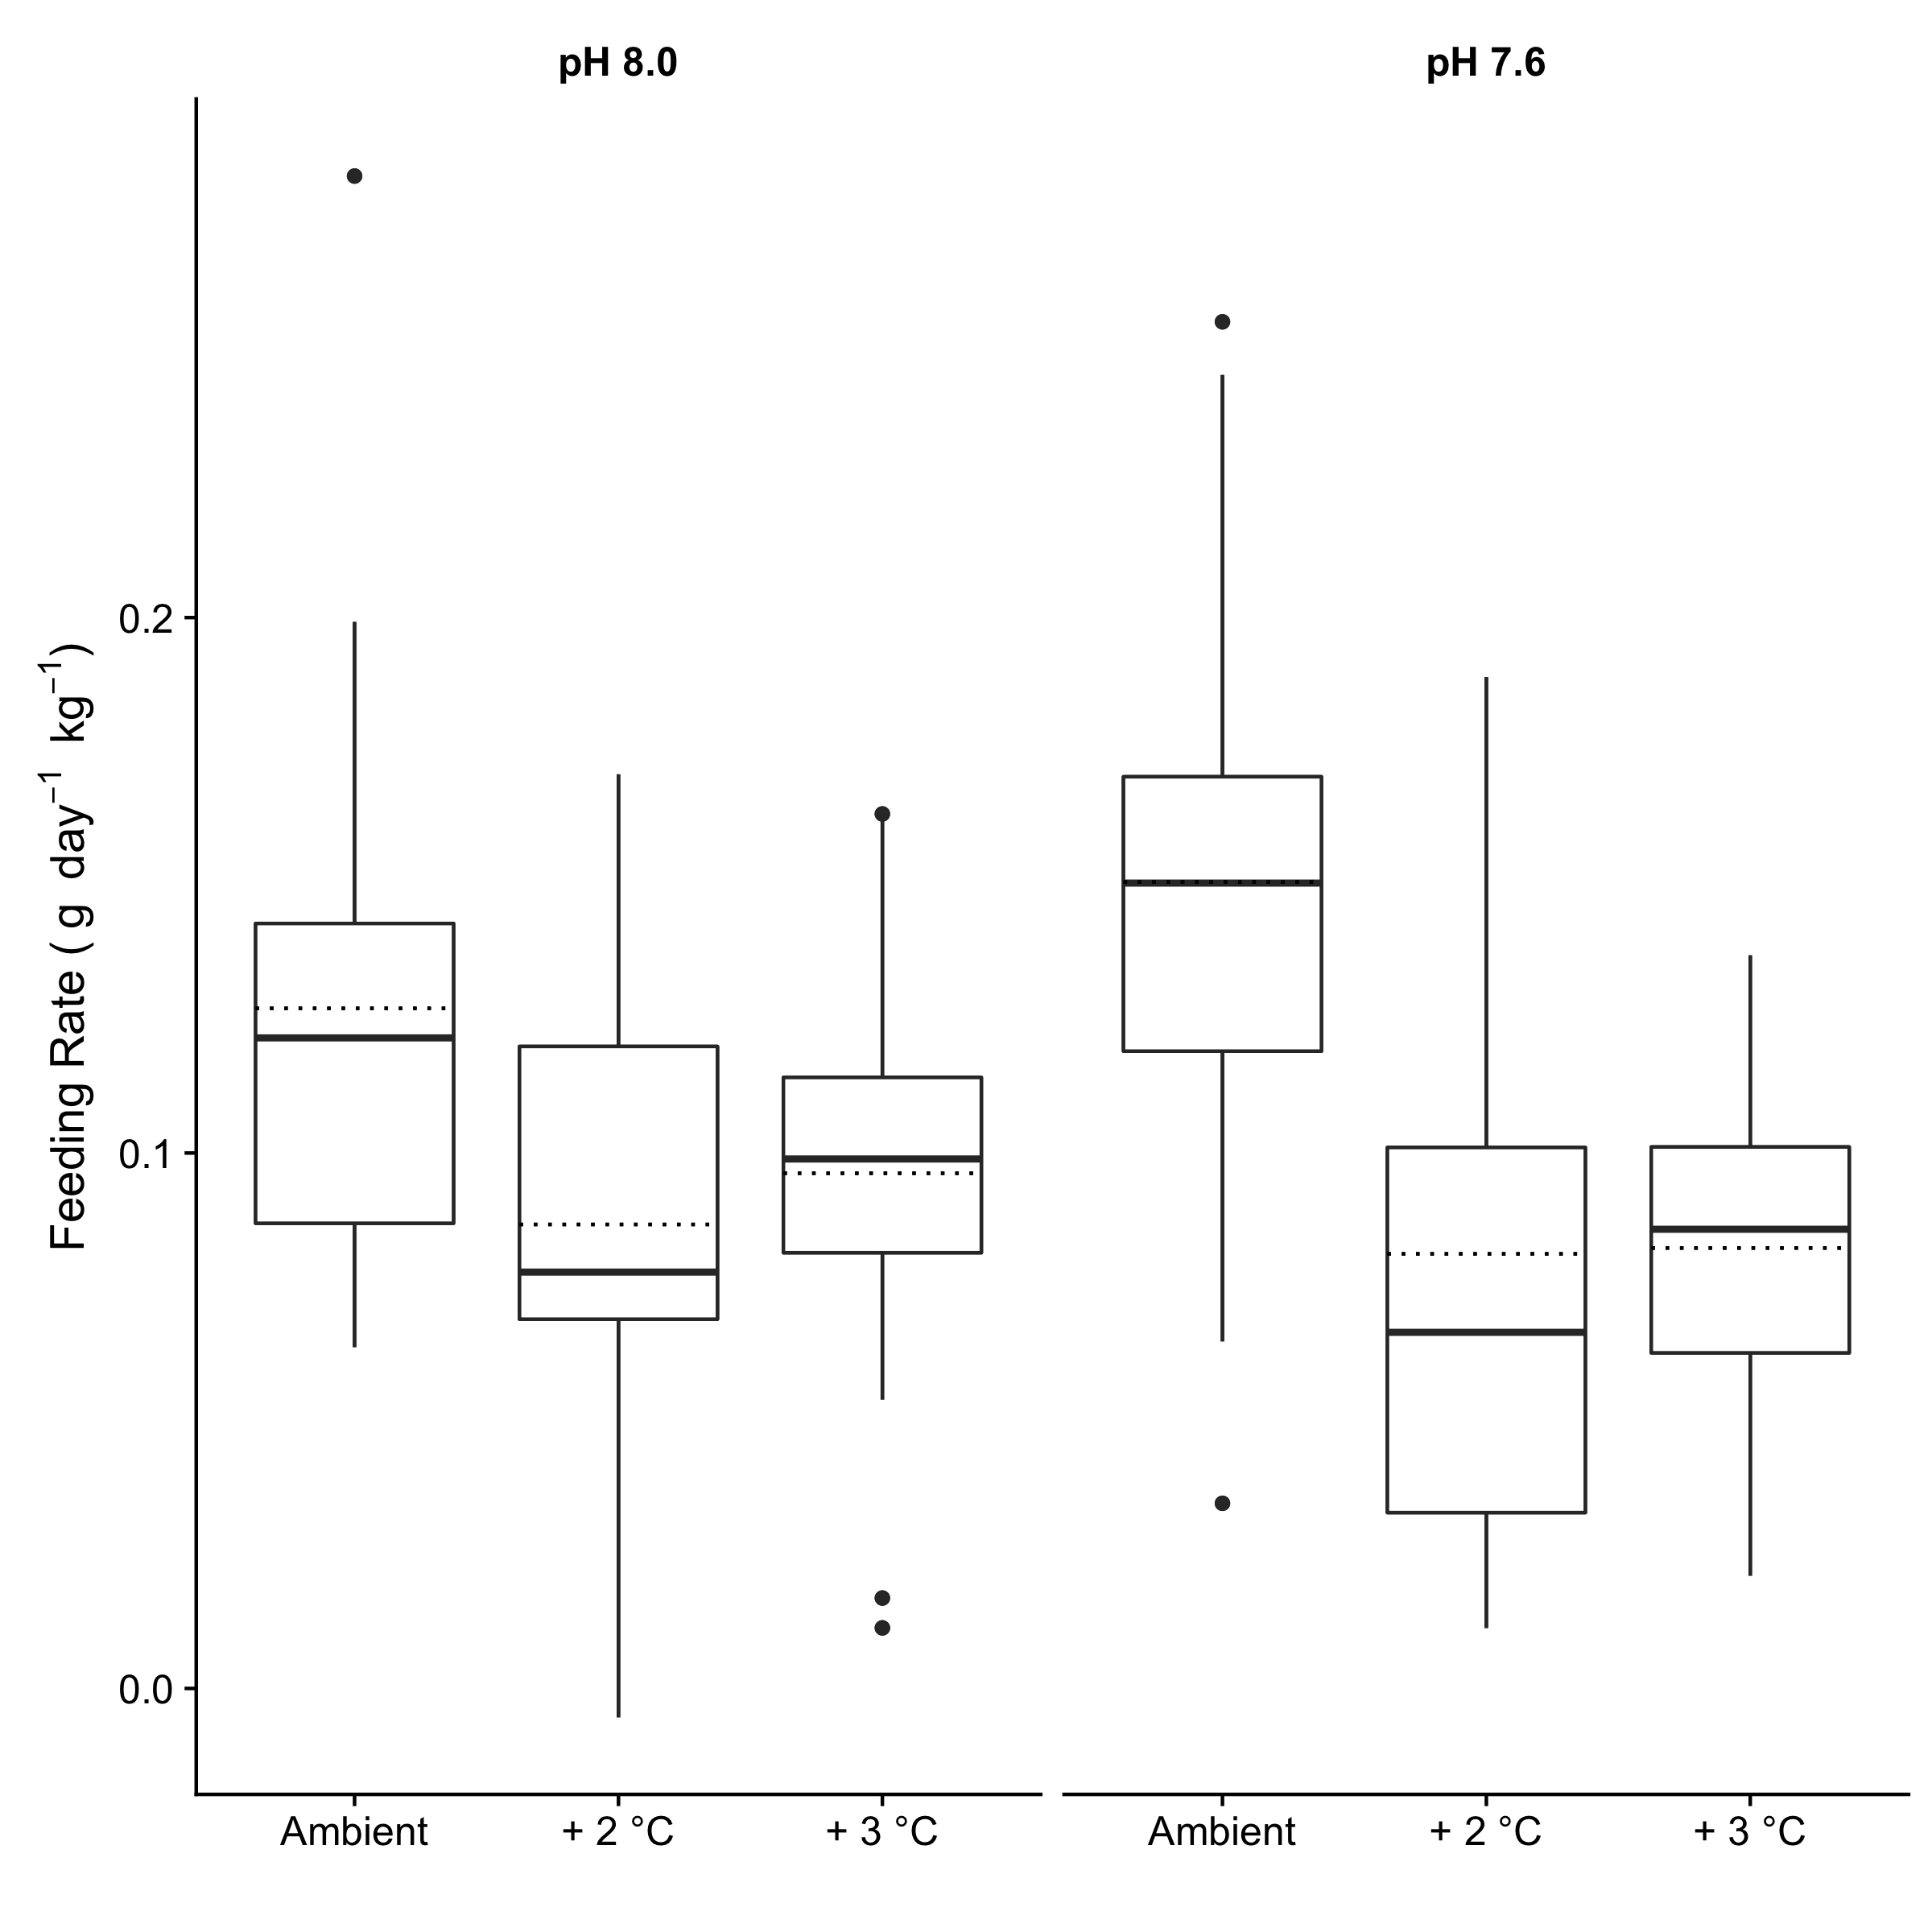
\includegraphics[width=1\linewidth]{figs/ch_multistressor/feed_plot} \caption{Feeding rate of *H. erythrogramma* acclimated for 12 weeks to conditions of increased temperature ($+0, +2, +3 ^\circ C$) and decreased pH (8.0, 7.6). The top and bottom of the boxes represent the interquartile range (IQR) between the 25th and 75th percentile (Q1 and Q3, respectively). The horizontal line represents the median (Q2), the horizontal dotted line represents the mean, and the vertical lines (whiskers) represent the range of the data computed as follows: Q1 − 1.5IQR (bottom whisker); greater than Q3 + 1.5 IQR (top whisker).}\label{fig:unnamed-chunk-5}
\end{figure}

\subsection{Ammonia excretion rate}\label{ammonia-excretion-rate}

Urchins acclimated to elevated temperature treatments had significantly
higher ammonia excretion rates (2-Way ANOVA, \(F_{1, 56} = 17.9\),
\(p < 0.001\)). Decreased pH had no significant effect
(\(F_{1, 56} = 0.92\), \(p < 0.34\)), and both temperature and pH did
not significantly interact (\(F_{1, 56} = 0.67\), \(p = 0.42\)).
\emph{Post-hoc} using Tukey's HSD (\(p = 0.05\)) showed that at ambient
pH (8.0), acclimation to \(+2 ^\circ C\) increased ammonia excretion by
1.3\(\times\) (\(d.f. =\) 54, \(p =\) 0.016), but not at \(+3 ^\circ C\)
(\(p =\) 0.099). At low pH (7.6), acclimation to \(+2 ^\circ C\) did not
significantly affect ammonia excretion (\(p =\) 0.29), but at
\(+3 ^\circ C\), excretion increased by 1.5\(\times\) (\(p =\) 0.016).

\begin{Shaded}
\begin{Highlighting}[]
\KeywordTok{load}\NormalTok{(}\StringTok{"output/ch_multistressor/ammonia.RData"}\NormalTok{)}
\NormalTok{hsd}\OperatorTok{$}\NormalTok{contrasts}
\end{Highlighting}
\end{Shaded}

\begin{verbatim}
## ph = 7.6:
##  contrast estimate       SE df t.ratio p.value
##  0 - 2      -14.34 9.442193 54  -1.519  0.2903
##  0 - 3      -35.80 9.442193 54  -3.791  0.0011
##  2 - 3      -21.46 9.442193 54  -2.273  0.0684
## 
## ph = 8.0:
##  contrast estimate       SE df t.ratio p.value
##  0 - 2      -27.05 9.442193 54  -2.865  0.0161
##  0 - 3      -19.84 9.442193 54  -2.101  0.0991
##  2 - 3        7.21 9.442193 54   0.764  0.7268
## 
## P value adjustment: tukey method for comparing a family of 3 estimates
\end{verbatim}

\begin{Shaded}
\begin{Highlighting}[]
\NormalTok{grps}\OperatorTok{$}\NormalTok{contrasts}
\end{Highlighting}
\end{Shaded}

\begin{verbatim}
##   contrast  ph estimate       SE df    t.ratio    p.value .group
## 2    0 - 3 7.6   -35.80 9.442193 54 -3.7914920 0.00108953      1
## 3    2 - 3 7.6   -21.46 9.442193 54 -2.2727770 0.06837392      1
## 1    0 - 2 7.6   -14.34 9.442193 54 -1.5187149 0.29027985      1
## 4    0 - 2 8.0   -27.05 9.442193 54 -2.8648005 0.01609529     12
## 5    0 - 3 8.0   -19.84 9.442193 54 -2.1012067 0.09907615     1 
## 6    2 - 3 8.0     7.21 9.442193 54  0.7635938 0.72675230      2
\end{verbatim}

\begin{Shaded}
\begin{Highlighting}[]
\NormalTok{knitr}\OperatorTok{::}\KeywordTok{include_graphics}\NormalTok{(}\StringTok{"figs/ch_multistressor/nh_plot.png"}\NormalTok{)}
\end{Highlighting}
\end{Shaded}

\begin{figure}
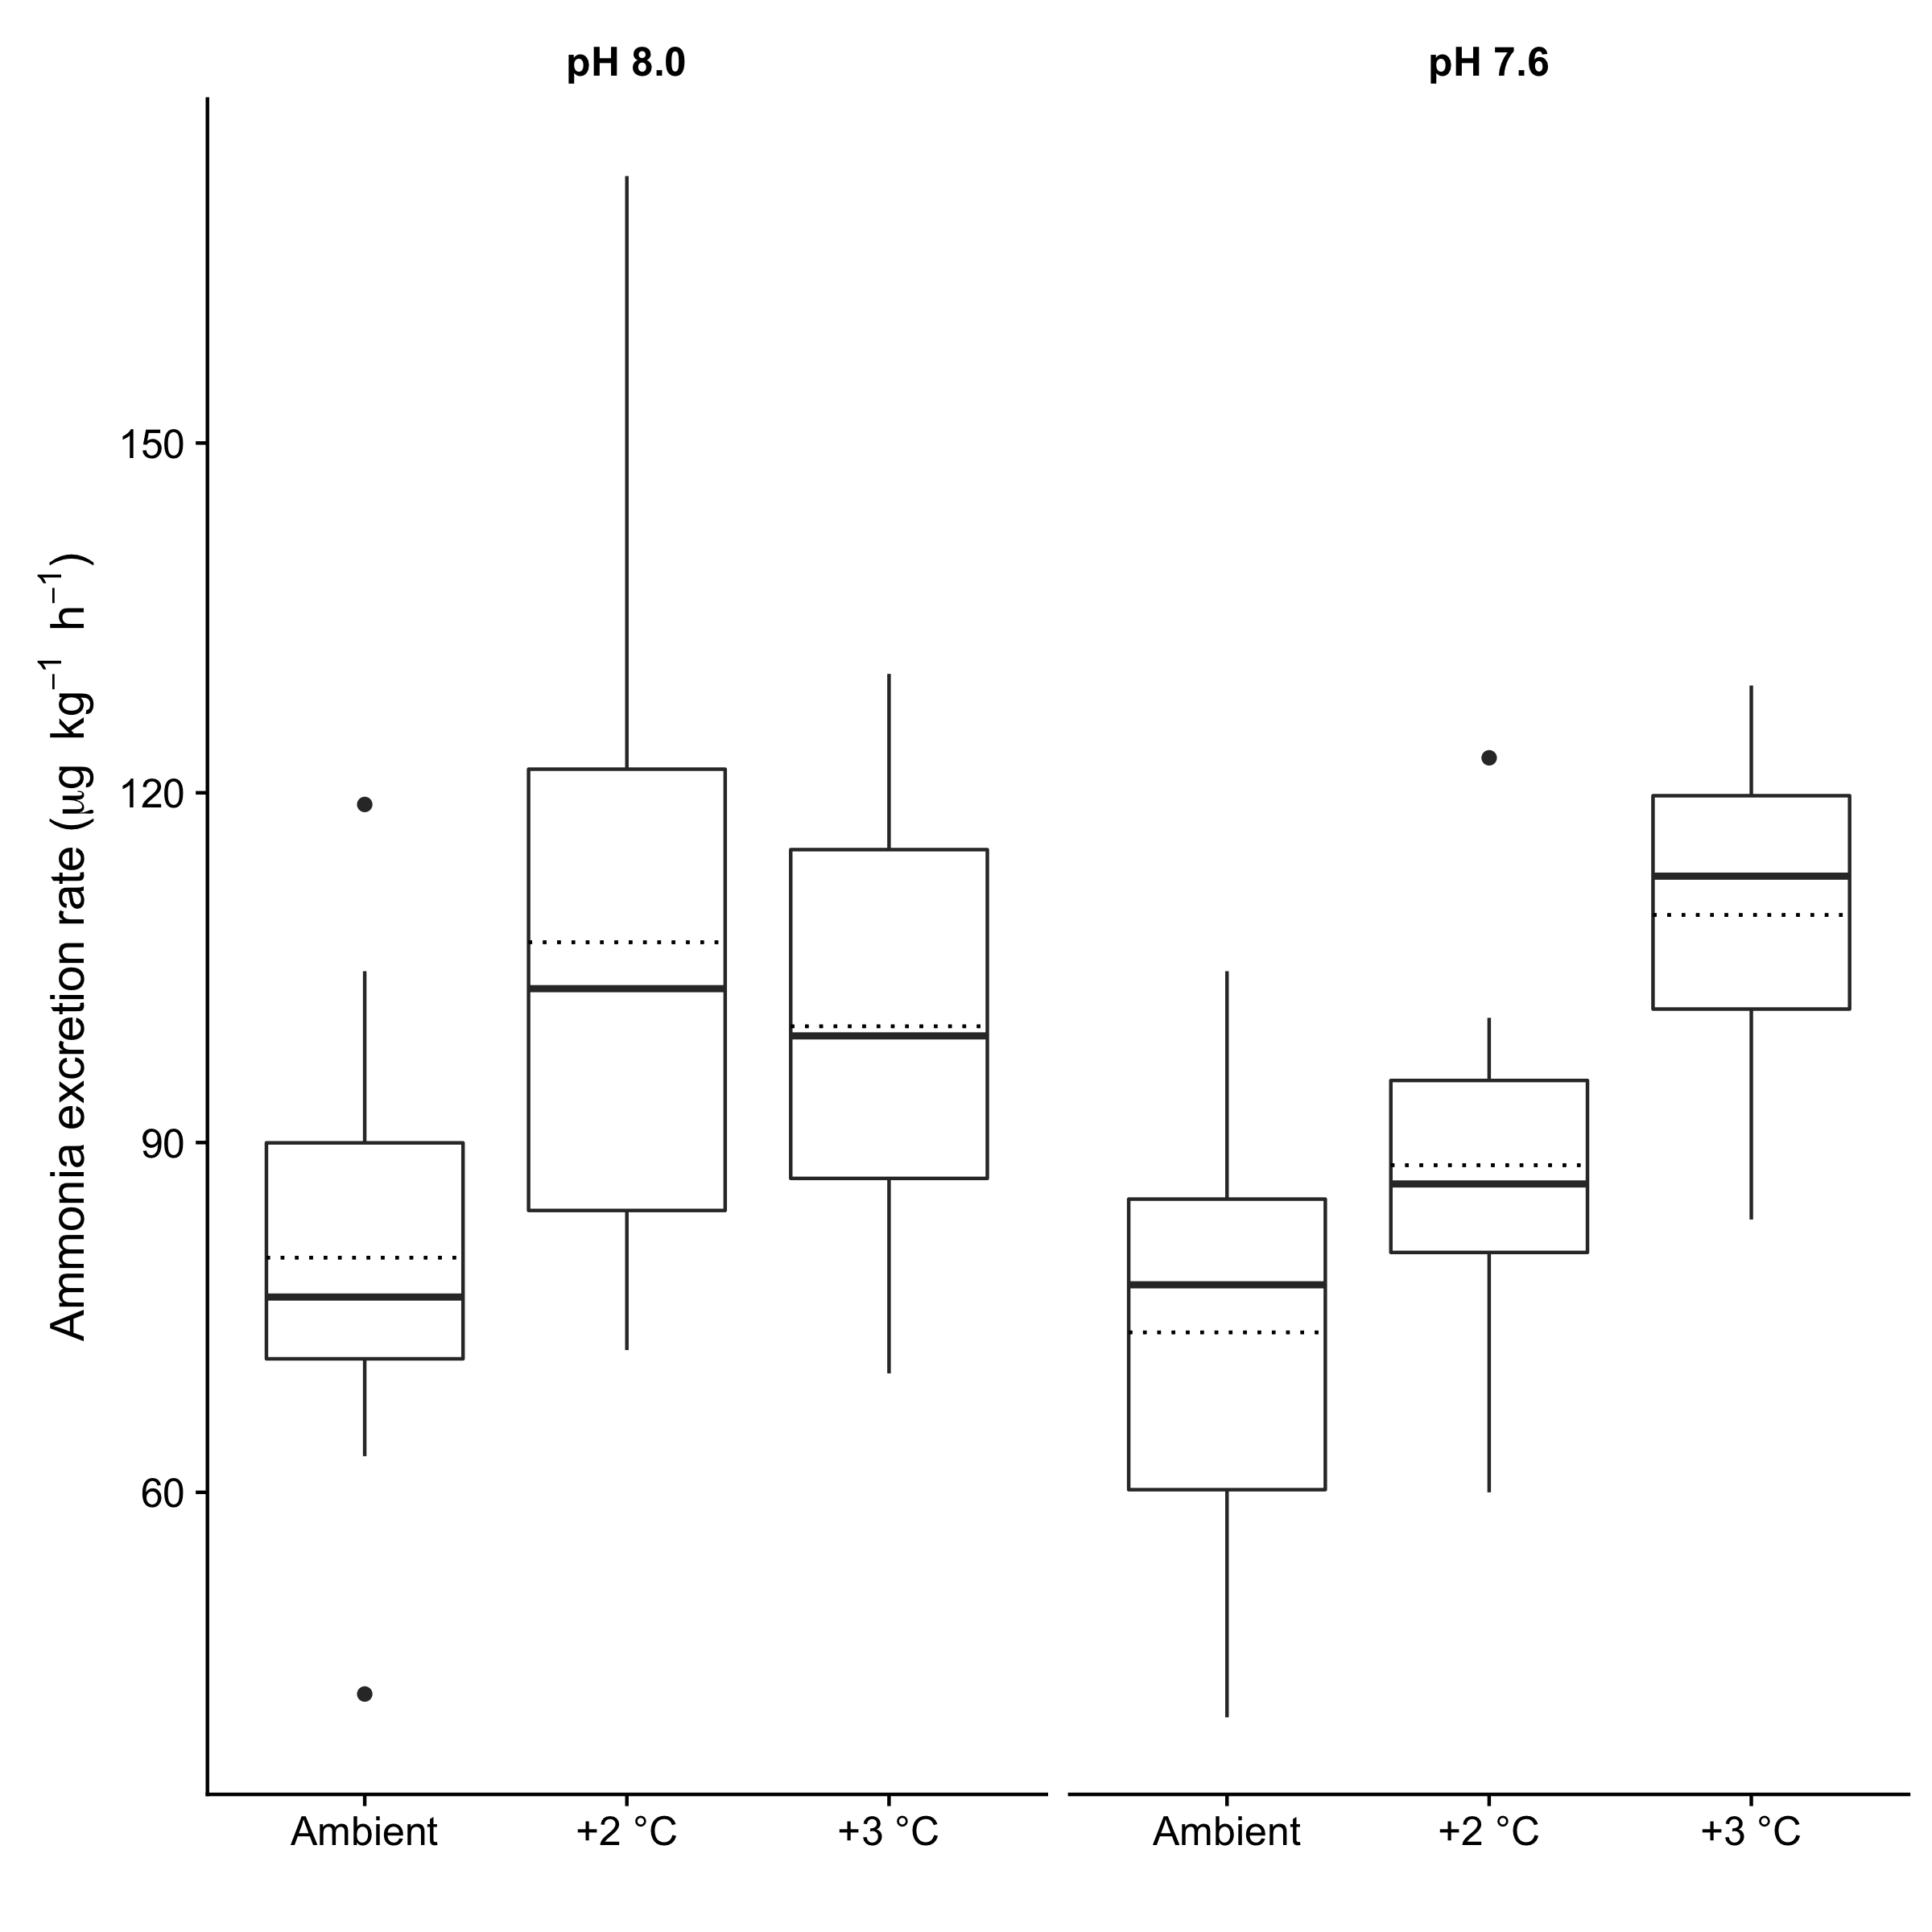
\includegraphics[width=1\linewidth]{figs/ch_multistressor/nh_plot} \caption{Feeding rate of *H. erythrogramma* acclimated for 12 weeks in six treatments of three temperatures ($+0, +2, +3 ^\circ C$) and two pH levels (8.0, 7.6). The top and bottom of the boxes represent the interquartile range (IQR) between the 25th and 75th percentile (Q1 and Q3, respectively). The horizontal line represents the median (Q2), the horizontal dotted line represents the mean, and the vertical lines (whiskers) represent the range of the data computed as follows: Q1 − 1.5IQR (bottom whisker); greater than Q3 + 1.5 IQR (top whisker).}\label{fig:unnamed-chunk-7}
\end{figure}

\subsection{Scope for growth}\label{scope-for-growth}

The SfG model for \emph{H. erythrogramma} indicated a negative
relationship between increased temperature and SfG. The highest SfG of
\(1.17 au\) was recorded for urchins in the ambient temperature \(+\)
low pH treatment.

\begin{Shaded}
\begin{Highlighting}[]
\NormalTok{sfg_table <-}\StringTok{ }\KeywordTok{as.data.frame}\NormalTok{(readxl}\OperatorTok{::}\KeywordTok{read_excel}\NormalTok{(}\StringTok{"figs/ch_multistressor/sfg_table.xlsx"}\NormalTok{))}
\NormalTok{sfg_table}
\end{Highlighting}
\end{Shaded}

\begin{verbatim}
##   Treatment    A   Ce    Re      Ue   SfG
## 1        0a 67.7 1.91 0.124 0.00184 1.170
## 2        0c 65.8 1.61 0.105 0.00200 0.953
## 3        2a 68.5 1.04 0.113 0.00220 0.599
## 4        2c 67.9 1.22 0.112 0.00268 0.714
## 5        3a 66.7 1.03 0.102 0.00274 0.582
## 6        3c 67.4 1.10 0.114 0.00250 0.623
\end{verbatim}

\begin{Shaded}
\begin{Highlighting}[]
\NormalTok{knitr}\OperatorTok{::}\KeywordTok{include_graphics}\NormalTok{(}\StringTok{"figs/ch_multistressor/sfg_plot.png"}\NormalTok{)}
\end{Highlighting}
\end{Shaded}

\begin{figure}
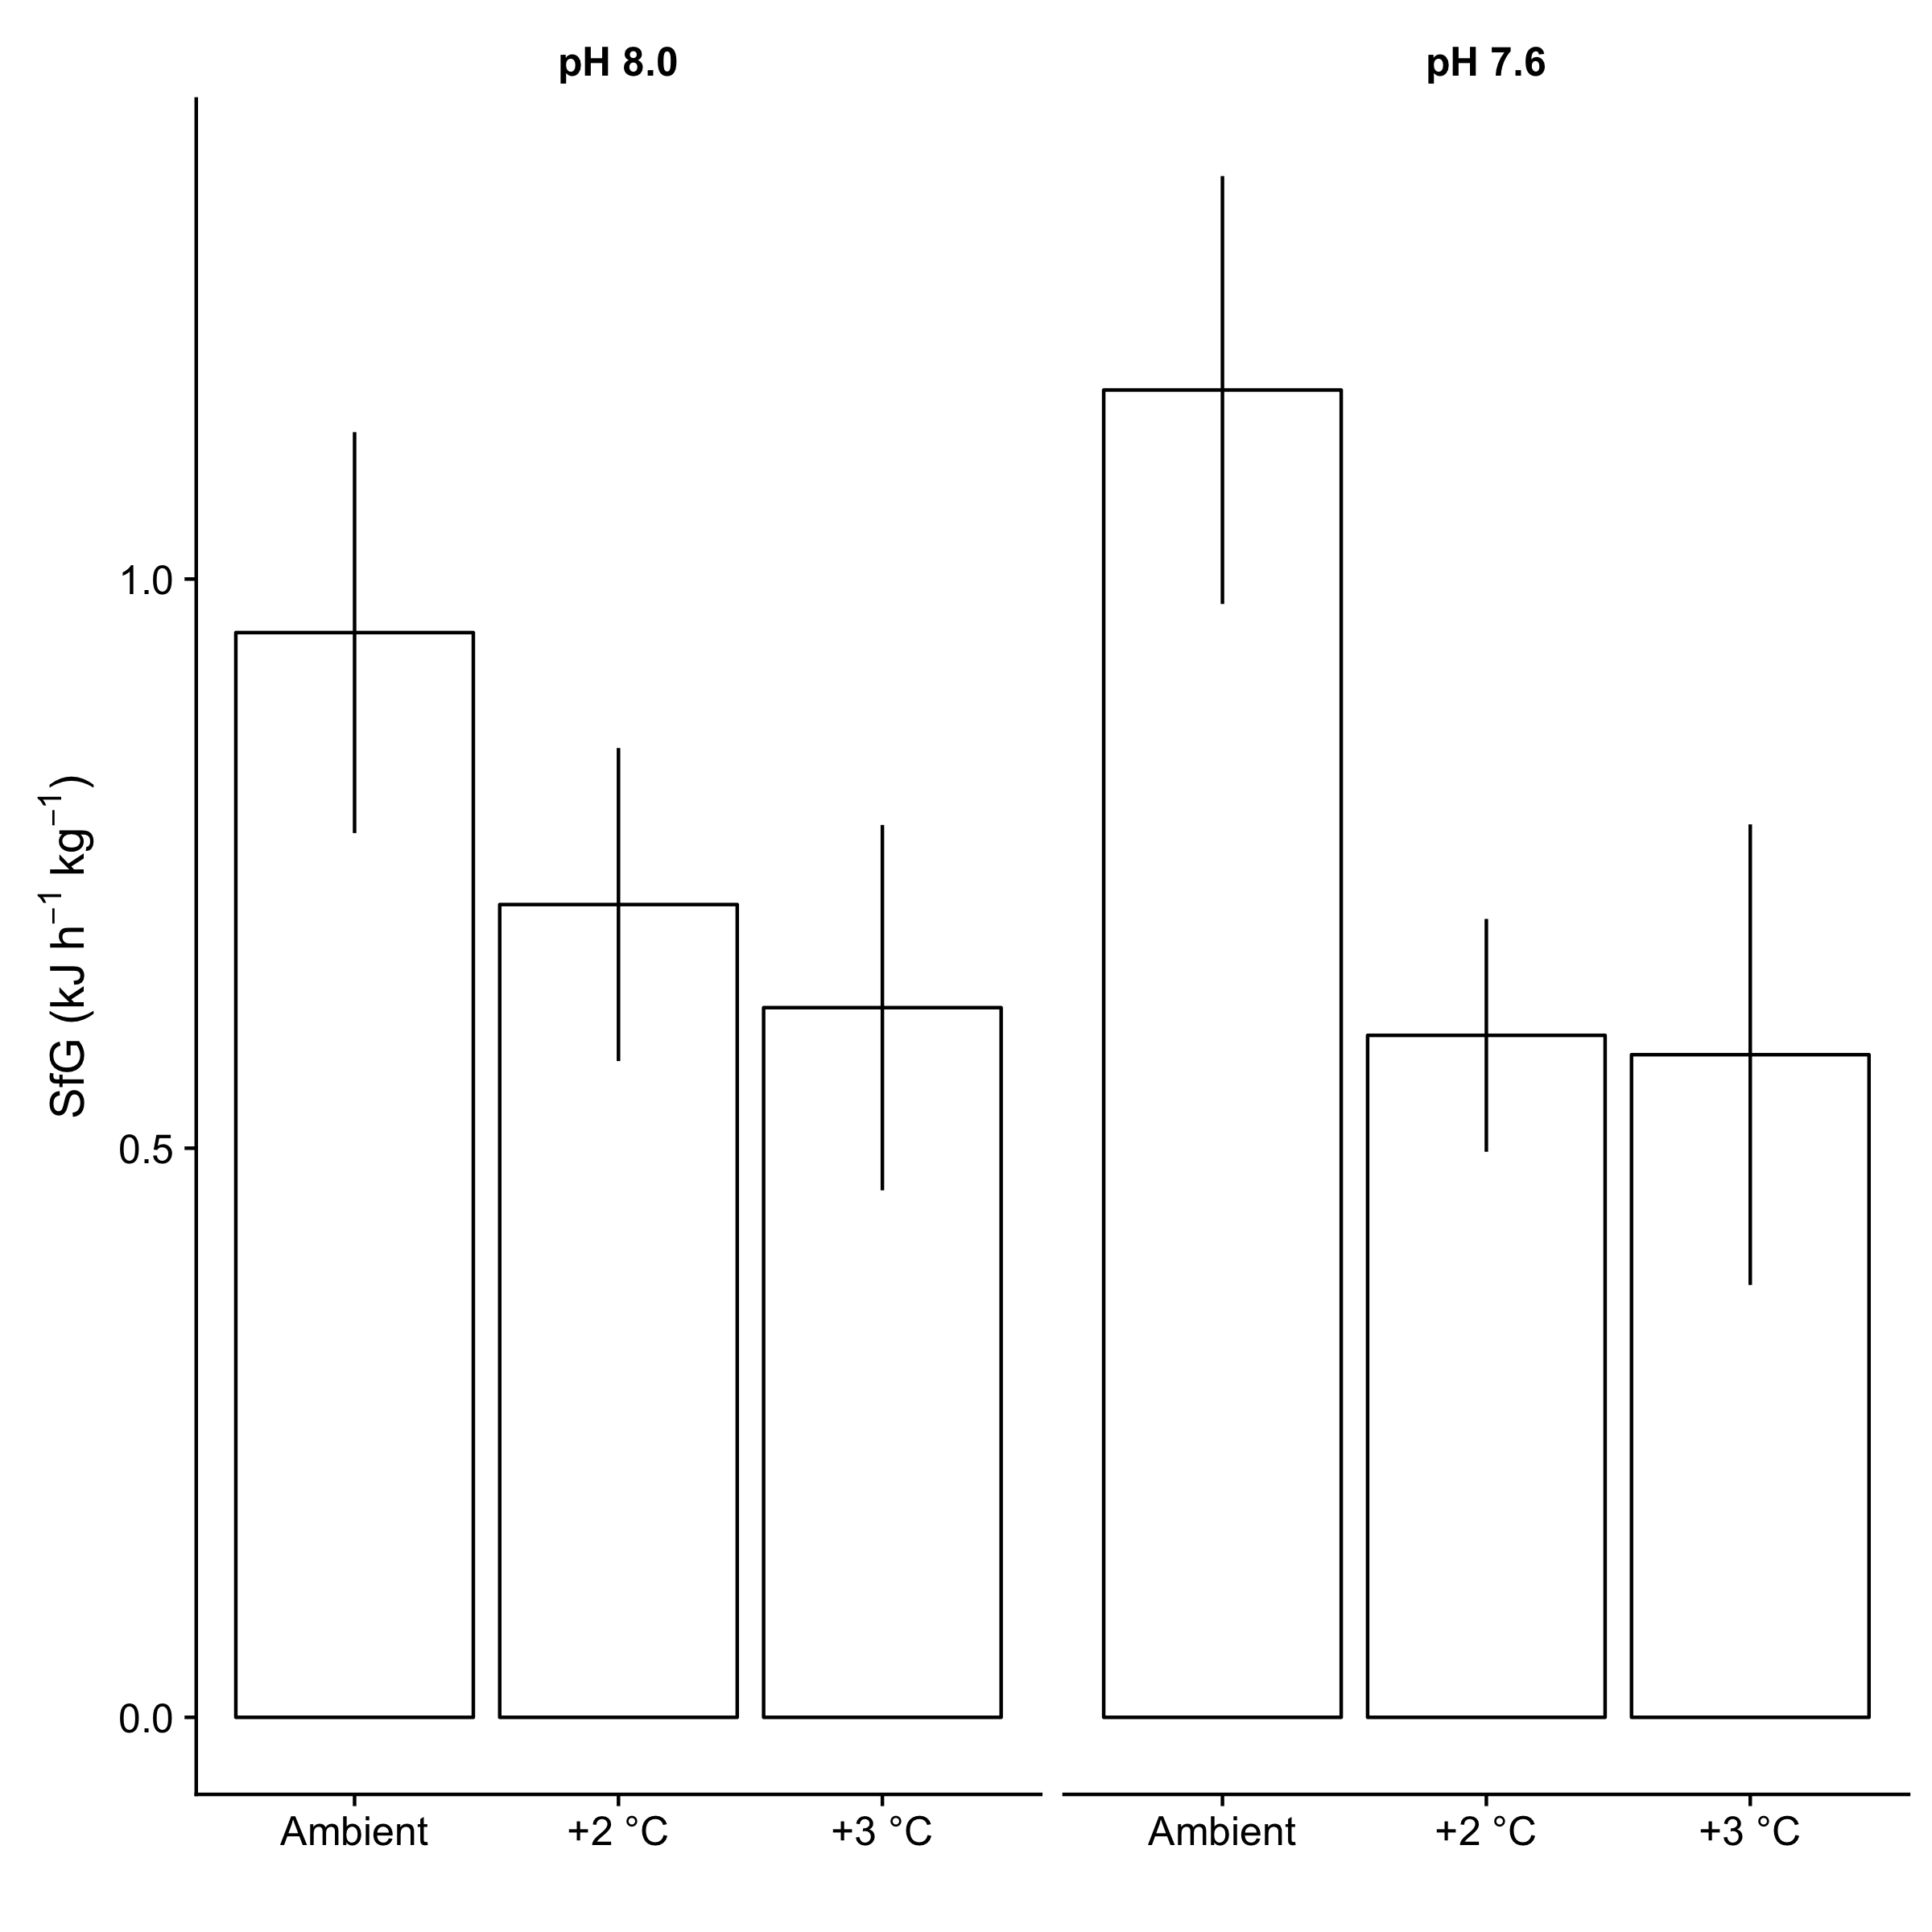
\includegraphics[width=1\linewidth]{figs/ch_multistressor/sfg_plot} \caption{Scope for growth ($\pm s.d.$) in the sea urchin, *H. erythrogramma* acclimated to conditions of increased temperature ($+0, +2, +3 ^\circ C$) and decreased pH (8.0, 7.6). }\label{fig:unnamed-chunk-9}
\end{figure}

\chapter{Methods}\label{methods-1}

We describe our methods in this chapter.

\chapter{Applications}\label{applications}

Some \emph{significant} applications are demonstrated in this chapter.

\section{Example one}\label{example-one}

\section{Example two}\label{example-two}

\chapter{Final Words}\label{final-words}

We have finished a nice book.

\bibliography{book.bib,packages.bib}


\end{document}
